\documentclass[oneside,a4paper,12pt]{article}


\usepackage[T1]{fontenc}
\usepackage[utf8]{inputenc}
\usepackage[english,polish]{babel} 
\usepackage[T1]{polski}
\usepackage{lmodern} % Wymagane przez microtype do działania ze skalowalnymi fontami w kodowaniu T1
\usepackage{mathptmx}
\DeclareMathAlphabet{\mathcal}{OMS}{cmsy}{m}{n} % Przywraca standardowy, ładny wygląd \mathcal
\usepackage{microtype} % Poprawia skład tekstu i eliminuje Overfull \hbox
\usepackage{graphicx}
\usepackage{color}
\usepackage{geometry}
\usepackage{url}
\usepackage{xurl}
\usepackage[hidelinks]{hyperref}
\usepackage{minted}
\usepackage{float}
\usepackage{amsmath}
\usepackage{amssymb}
\usepackage{csquotes}
\usepackage{tikz}
\usetikzlibrary{shapes, positioning, arrows.meta}

\usepackage[
    backend=biber,
    style=verbose-trad1,
    citestyle=verbose-trad1,
    autocite=footnote,
    sorting=nyt,
    giveninits=false,
    maxnames=3,
    minnames=1,
    date=year,
    doi=false,
    isbn=false,
    url=false,
    eprint=false
]{biblatex}
\addbibresource{Moja biblioteka.bib}

% --- REGULAMINOWE ZASADY CYTOWANIA W PRZYPISACH ---
\DeclareNameAlias{default}{given-family}
\DeclareNameAlias{sortname}{given-family}

% 1. Czasopisma: Tytuł artykułu w cudzysłowach, nazwa czasopisma kursywą
\DeclareFieldFormat[article]{title}{\enquote{#1}}
\DeclareFieldFormat[article]{journaltitle}{\mkbibemph{#1}\isdot}
\DeclareFieldFormat[article]{volume}{t.~#1}
\DeclareFieldFormat[article]{number}{nr~#1}

\renewbibmacro*{journal+issuetitle}{%
  \usebibmacro{journal}%
  \setunit*{\addcomma\space}%
  \usebibmacro{date}%
  \setunit{\addcomma\space}%
  \printfield{volume}%
  \setunit{\addcomma\space}%
  \printfield{number}%
  \setunit{\addcomma\space}%
  \printfield{eid}%
  \setunit{\addcomma\space}%
  \usebibmacro{issue}%
  \newunit}
\renewbibmacro*{issue+date}{}

% 2. Prace zbiorowe: (w:) Tytuł książki
\DeclareFieldFormat[incollection]{title}{#1}
\DeclareFieldFormat[incollection]{booktitle}{#1}

% 3. Formatowanie stron, dat i symboli w przypisach
\AtEveryBibitem{\clearfield{month}\clearfield{day}}
\DeclareFieldFormat{postnote}{s.~#1}
\DeclareFieldFormat{pages}{s.~#1}

% Zamiana domyślnych kropek oddzielających sekcje w przypisie na przecinki
\renewcommand*{\newunitpunct}{\addcomma\space}

\DefineBibliographyStrings{polish}{
  ibidem = {Ibidem},
  loccit = {Ibidem},
  andothers = {i~in\adddot}
}

% Usunięcie "W:" lub "(w:)" przed tytułami czasopism i prac zbiorowych
\renewbibmacro{in:}{}

% --- ZARZĄDZANIE ŹRÓDŁAMI INTERNETOWYMI ---
\DeclareSourcemap{
  \maps[datatype=bibtex]{
    \map{
      \pertype{misc}
      \step[fieldsource=howpublished, match=\regexp{^https?://}, final]
      \step[fieldset=keywords, fieldvalue=internet, append]
      \step[typesource=misc, typetarget=online]
    }
    \map{
      \pertype{misc}
      \step[fieldsource=url, match=\regexp{^https?://}, final]
      \step[fieldset=keywords, fieldvalue=internet, append]
      \step[typesource=misc, typetarget=online]
    }
  }
}

\DeclareFieldFormat[online]{urldate}{\mkbibparens{\bibstring{urlseen}\space#1}}

\DeclareBibliographyDriver{online}{%
  \iffieldundef{howpublished}
    {\printfield{url}}
    {\printfield{howpublished}}%
  \setunit{\space}%
  \iffieldundef{urlyear}
    {}
    {\printurldate}%
  \finentry
}



\geometry{left=3.5cm, right=2.5cm, top=2.5cm, bottom=2.5cm}
\raggedbottom
\usepackage{epstopdf}

% --- FORMATOWANIE AKAPITÓW, BIBLIOGRAFII I PRZYPISÓW DOLNYCH ---
\usepackage{indentfirst}
\setlength{\parindent}{0.75cm}
\setlength{\parskip}{0pt plus 1pt}
\setlength{\bibhang}{0.75cm}

\usepackage[hang,bottom,multiple]{footmisc}
\setlength{\footnotemargin}{0.8em}
\setlength{\skip\footins}{1.8em plus 0.5em minus 0.2em}

\usepackage{multicol}
%\usepackage[toc,page]{appendix}
\usepackage{caption}
\captionsetup{labelfont=bf, labelsep=colon, justification=raggedright, singlelinecheck=false}

%\usepackage{emptypage}
%\pretocmd{\section}{\cleardoublepage}{}{}

\usepackage{multirow}

% --- DODANIE KROPKI PO NUMERZE SEKCJI ---
\usepackage{titlesec}
\titlelabel{\thetitle.\quad}

\newcommand{\setSupervisor}[1]{
    \newcommand{\supervisor}{#1}
}
\newcommand{\setFaculty}[1]{
    \newcommand{\faculty}{#1}
}

\newcommand{\setDepartment}[1]{
    \newcommand{\department}{#1}
}

\newcommand{\setReviewer}[1]{
    \newcommand{\reviewer}{#1}
}

\newcommand{\setTitleang}[1]{
    \newcommand{\Titleang}{#1}
}

\newcommand{\setMajor}[1]{
    \newcommand{\major}{#1}
}


\makeatletter
\renewcommand{\maketitle}{\begin{titlepage}
        \begin{center}
            
\includegraphics[height=60.85mm]{img/agh_nzw_s_pl_1w_wbr_rgb_150ppi.jpg}\\
        \end{center}
        %\rule{30mm}{0pt}

        \begin{center}
            {\normalsize \bfseries \sffamily \MakeUppercase{\faculty}}\\
            \vspace{1ex}
            {\normalsize \sffamily \MakeUppercase{\department}}\\
        \end{center}
        \vspace{7.5ex}


        \begin{center}
            {\Large \textsf{Praca dyplomowa}}\\
            \vspace{8ex} % Zmniejszono z 13ex, żeby podnieść tytuł wyżej
            %% ------------------------ TYTUł PRACY --------------------------------------
            {\bf \Large \textsf{\@title}}\\
            \vspace{3ex}
            {\large \textsf{\Titleang}}\\
        \end{center}

        % DODANO \vfill - elastyczna sprężyna, która spycha resztę na sam dół strony
        \vfill

        %\begin{left}
        % --------------------------- IMIE I~NAZWISKO -------------------------------
        \noindent
        {\normalsize \bf \textsf{Autor:}} {\normalsize \textsf{\@author}}\\[1.5ex]
        \noindent
        {\normalsize \bf \textsf{Kierunek studiów:}} {\normalsize \textsf{\major}}\\[1.5ex]
        \noindent
        {\normalsize \bf \textsf{Opiekun:}} {\normalsize \textsf{\supervisor}}
        \vspace{4ex}

        \begin{center}
            {\normalsize \textsf{Kraków, 2026}}
        \end{center}

    \end{titlepage}%
}
\makeatother 

% ---TU WPISZ IMIĘ I NAZWISKO -----
\author{Jakub Sornat}

% --- TU WPISZ TYTUŁ PRACY
\title{Porównanie algorytmów rekomendacyjnych
(Filtrowanie Kolaboracyjne, Uczenie Głębokie, Grafowe Sieci Neuronowe) na przykładzie portalu streamingowego
}
% LTeX: enabled=false
\setTitleang{Comparison of recommendation algorithms
(Collaborative Filtering, Deep Learning, Graph Neural Networks) using a streaming platform as an example
}
% LTeX: enabled=true


% --- TU WPISZ KIERUNEK STUDIÓW
\setMajor{Informatyka i Ekonometria}

\setDepartment{Katedra Informatyki Biznesowej i Inżynierii Zarządzania}
\setFaculty{Wydział Zarządzania}
\setSupervisor{dr hab. Iwona Skalna}

\begin{document}
\pagestyle{empty}

\renewcommand\refname{Bibliografia}

\maketitle

\pagestyle{plain}
\linespread{1.3}
\selectfont

\newpage
\pagenumbering{roman}
\tableofcontents

\newpage

\pagenumbering{arabic}

% !TEX root = ../PRACA_MAIN.tex
\section*{Wstęp} \addcontentsline{toc}{section}{Wstęp}
W dobie dynamicznego rozwoju platform cyfrowych, a w szczególności serwisów oferujących wideo na żądanie (VOD), użytkownicy coraz częściej stykają się ze zjawiskiem przeciążenia poznawczego. Ilość dostępnych treści znacznie przekracza ludzkie możliwości poznawcze i analityczne, a proces wyboru interesujących treści staje się dla użytkownika czasochłonny i mało efektywny. W takich warunkach systemy rekomendacyjne stają się nie tylko udogodnieniem, ale wręcz kluczowym narzędziem nawigacyjnym oraz podstawowym mechanizmem budowania zaangażowania i satysfakcji klienta. Dynamiczny rozwój metod sztucznej inteligencji doprowadził do powstania wielu zaawansowanych algorytmów rekomendacyjnych. Główną motywacją do podjęcia niniejszej tematyki jest chęć sprawdzenia, który z analizowanych sposobów generowania rekomendacji najlepiej sprawdzi się w przyjętym środowisku badawczym i przy określonych kryteriach oceny.

W pracy przeanalizowano cztery modele rekomendacyjne: algorytm oparty na sąsiedztwie obiektów (ItemKNN), klasyczną faktoryzację macierzy optymalizowaną za pomocą spersonalizowanego rankingu bayesowskiego (ang. \foreignlanguage{english}{\textit{Bayesian Personalized Ranking}} -- BPR-MF), neuronowe filtrowanie kolaboracyjne (ang. \foreignlanguage{english}{\textit{Neural Collaborative Filtering}} -- NCF) oraz algorytm LightGCN, reprezentujący grafowe sieci neuronowe (ang. \foreignlanguage{english}{\textit{Graph Neural Networks}}). Zostały one dobrane w taki sposób, aby zilustrować kluczowe kierunki rozwoju systemów tego typu. ItemKNN oraz BPR-MF to klasyczne techniki filtrowania kolaboracyjnego, stanowiące główny punkt odniesienia. Z kolei NCF opiera się na architekturach uczenia głębokiego (ang. \foreignlanguage{english}{\textit{Deep Learning}}). LightGCN natomiast bada potencjał wspomnianych wcześniej struktur grafowych. Takie zestawienie umożliwia bezpośrednie porównanie tradycyjnych fundamentów z nowocześniejszymi rozwiązaniami. Zakres badań obejmuje opis teoretyczny, implementację w środowisku eksperymentalnym oraz ocenę skuteczności poszczególnych podejść.

Celem badawczym jest ocena przewagi metod rekomendacyjnych opartych na głębokich sieciach neuronowych i strukturach grafowych nad klasycznymi metodami filtrowania kolaboracyjnego oraz analiza relacji pomiędzy jakością predykcji a złożonością obliczeniową tych metod.

W realizacji pracy wykorzystano zróżnicowane źródła informacji. Warstwa teoretyczna opiera się głównie na anglojęzycznej i polskiej literaturze przedmiotu. Podstawę stanowiły recenzowane artykuły naukowe oraz publikacje z wiodących konferencji poświęconych sztucznej inteligencji. Materiał badawczy stanowił powszechnie uznawany zbiór danych MovieLens\footcite{MovieLens2013}, który dobrze odzwierciedla charakterystykę preferencji użytkowników platform filmowych. Dokumentacja techniczna dedykowanych bibliotek (w tym frameworku RecBole) stanowiła bazę informacyjną do implementacji badanych architektur.

W przeprowadzonych badaniach oparto się na praktycznej implementacji modeli oraz ilościowej ocenie ich skuteczności. Zastosowano zaawansowane strojenie hiperparametrów algorytmów z użyciem techniki przeszukiwania siatki (ang. \foreignlanguage{english}{\textit{Grid Search}}) oraz eksperymenty analizujące zbieżność funkcji straty w procesie uczenia. Do oceny jakości generowanych rekomendacji zastosowano ugruntowane w dziedzinie metryki ewaluacyjne, takie jak znormalizowany zdyskontowany zysk skumulowany (ang. \foreignlanguage{english}{\textit{Normalized Discounted Cumulative Gain}} -- NDCG) czy wskaźnik trafień (ang. \foreignlanguage{english}{\textit{Hit Rate}} -- HR). Modele zaimplementowano i przetrenowano w środowisku języka Python. Realizacja założonego celu podyktowała podział pracy na trzy rozdziały.

Rozdział pierwszy stanowi wprowadzenie w problematykę systemów rekomendacyjnych. Omówiono w nim specyfikę serwisów VOD, zdefiniowano niezbędne pojęcia, przedstawiono formalizm matematyczny, a także zarysowano ewolucję paradygmatów personalizacji treści. Przedstawiono również kluczowy dla rozważanej tematyki przegląd dotychczasowej literatury oraz zdefiniowano główne wyzwania badawcze.

Rozdział drugi poświęcono metodyce badawczej oraz szczegółowemu opisowi testowanych algorytmów. Scharakteryzowano w nim wykorzystane środowisko wykonawcze i sposób przygotowania danych. Kolejna część rozdziału przybliża teoretyczne podstawy badanych modeli. Przedstawiono zasady ich działania oraz architekturę: od klasycznego filtrowania kolaboracyjnego, przez uczenie głębokie, aż po grafowe sieci neuronowe. Rozdział ten zamyka formalna definicja zastosowanych metryk oceny.

W rozdziale trzecim zaprezentowano właściwe rezultaty przeprowadzonych eksperymentów numerycznych i ich szczegółową analizę. Udokumentowano proces strojenia hiperparametrów, zestawiono algorytmy pod kątem jakości predykcji, zbadano koszty obliczeniowe i stabilność treningu. Praca kończy się dyskusją nad osiągniętymi wynikami i sformułowaniem wniosków płynących z badań.

% !TEX root = ../PRACA_MAIN.tex

\section{Wprowadzenie do problematyki systemów rekomendacyjnych}

Rozdział pierwszy przedstawia teoretyczne oraz rynkowe podstawy systemów rekomendacyjnych. Omówiono w nim zjawisko przeciążenia poznawczego na rynku platform VOD, formalny podział metod personalizacji treści oraz technologiczną ewolucję algorytmów -- od klasycznych podejść opartych na algebrze macierzy po zaawansowane struktury grafowe. Rozdział kończy analiza kluczowych wyzwań wdrożeniowych związanych z projektowaniem tego typu systemów.

\subsection{Zjawisko przeciążenia poznawczego i specyfika rynku VOD} % REVIEWED

Rozwój technologii internetowych w pierwszych dekadach XXI wieku doprowadził do cyfryzacji głównych segmentów rynku rozrywkowego. W sektorze wideo obserwuje się stopniowe odchodzenie od tradycyjnej telewizji na rzecz platform VOD. Rynek ten zdominowały serwisy globalne (np. Netflix, Max, Amazon Prime Video) oraz dostawcy lokalni (np. Player.pl, TVP VOD). Analogiczne zmiany nastąpiły w branży muzycznej, gdzie czołową pozycję zajmują platformy takie jak Spotify i Apple Music. Model subskrypcyjny wprowadzono także na rynku wydawniczym, umożliwiając stały dostęp do e-booków oraz audiobooków. W rezultacie użytkownicy mogą korzystać z obszernych baz multimedialnych z poziomu pojedynczej aplikacji.

Rosnąca objętość udostępnianych katalogów stanowi jednak istotny problem z perspektywy użytkownika. Ze względu na znaczną liczbę dostępnych materiałów, odbiorcy często doświadczają zjawiska przeciążenia poznawczego (ang. \foreignlanguage{english}{\textit{cognitive overload}}) \footcite{bollenUnderstandingChoiceOverload2010}. Zjawisko to występuje powszechnie w całym sektorze cyfrowej rozrywki, co potwierdzają dane rynkowe. Baza IMDb indeksuje ponad 30 milionów tytułów filmowych i telewizyjnych \footcite{PressRoomIMDb}. Katalog platformy Spotify obejmuje ponad 100 milionów utworów \footcite{AboutSpotify}, natomiast serwis BookBeat oferuje subskrybentom dostęp do ponad miliona pozycji literackich \footcite{BookBeatONas}.

Setki tysięcy produkcji w ramach pojedynczego serwisu wywołują u odbiorcy efekt tzw. paradoksu wyboru \footcite{schwartzParadoxChoiceWhy2005}. Nadmierna ekspozycja na treści przytłacza użytkownika, sprawiając, że całościowa eksploracja katalogu staje się fizycznie niemożliwa, a podjęcie decyzji o wyborze seansu wiąże się ze znacznym wysiłkiem poznawczym. Takie przeciążenie w wielu przypadkach prowadzi do zniechęcenia, frustracji widza, a ostatecznie do rezygnacji z subskrypcji. Rozwiązania tradycyjne, takie jak wyszukiwanie frazowe czy statyczne, redakcyjne zestawienia popularności, okazują się niewystarczające, ponieważ wymagają one aktywnej inicjatywy ze strony odbiorcy lub promują pozycje najpopularniejsze, nieuwzględniające jego indywidualnych preferencji \footcite{krawczukSystemyRekomendacyjne2024}.

W konsekwencji zaawansowane systemy rekomendacyjne przestały być jedynie opcjonalnym dodatkiem funkcjonalnym, stając się integralnym i kluczowym elementem architektury współczesnych platform cyfrowych \footcite[23--24]{Bernardelli2024}. Ich nadrzędnym zadaniem jest ciągłe, zautomatyzowane analizowanie ogromnych katalogów treści i filtrowanie ich w taki sposób, aby skutecznie chronić widza przed zjawiskiem paraliżu decyzyjnego. Zamiast zmuszać odbiorcę do samodzielnego przeszukiwania tysięcy tytułów, algorytmy te dostarczają spersonalizowane propozycje, ściśle dopasowane do jego profilu, historii oglądania oraz preferencji. W cyfrowym modelu biznesowym, opartym na miesięcznych subskrypcjach, to właśnie trafność tych podpowiedzi stanowi podstawowe narzędzie budujące lojalność i długoterminowe zaangażowanie użytkowników. Skuteczność takiego podejścia najlepiej obrazują wewnętrzne dane platformy Netflix, z których wynika, że precyzyjne sugestie algorytmiczne odpowiadają za wygenerowanie aż 80\% całkowitego czasu, jaki widzowie spędzają na odtwarzaniu materiałów w serwisie \footcite{gomez-uribeNetflixRecommenderSystem2015}.

\subsection{Definicje, formalizm matematyczny i struktura danych w personalizacji treści} % REVIEWED

W niniejszym podrozdziale wprowadzono podstawowe pojęcia pozwalające zrozumieć działanie systemów personalizacji treści. Przedstawiono rozwój oraz matematyczny zapis problemu rekomendacji, a także omówiono specyfikę danych wykorzystywanych przez współczesne algorytmy uczenia maszynowego.

\subsubsection{Ewolucja pojęcia systemów rekomendacji}

Historycznie pojęcie systemów rekomendacji ewoluowało wraz z postępującą cyfryzacją oraz narastającym problemem przeciążenia poznawczego. Pierwsze rozwiązania badawcze miały charakter ściśle kooperacyjny i opierały się na świadomej współpracy odbiorców. Pionierskim przykładem jest stworzony w 1992 roku przez badaczy z Xerox Palo Alto Research Center (PARC) system Tapestry \footcite{goldbergUsingCollaborativeFiltering1992}. Powstał on w odpowiedzi na dynamicznie rosnącą liczbę wiadomości w sieciach korporacyjnych i na grupach dyskusyjnych, proponując nowatorskie podejście do selekcji strumieni danych. Tapestry umożliwiał użytkownikom filtrowanie przychodzących dokumentów na podstawie jawnych, manualnych adnotacji i ocen wprowadzonych wcześniej przez innych czytelników (np. żądanie wyświetlania wyłącznie tych wiadomości, które konkretny współpracownik oznaczył jako wartościowe). To właśnie w publikacji opisującej ten system po raz pierwszy w literaturze sformułowano termin "filtrowanie kolaboracyjne", kładąc podwaliny pod cały współczesny nurt badań nad personalizacją treści. Chociaż system Tapestry działał zadowalająco, to jednak ze względu na wymóg budowania skomplikowanych zapytań i ograniczenie do małych, zamkniętych społeczności, w których użytkownicy znali się nawzajem, jego koncepcja szybko ewoluowała w stronę w pełni zautomatyzowanych, bezobsługowych algorytmów na dużą skalę.

Przełomowym momentem dla rozwoju pojęć w tej dziedzinie była praca opublikowana w 1997 roku przez P. Resnicka i H. Variana \footcite{RecommenderSystems1997}. Badacze ci zaproponowali, aby wąskie pojęcie "filtrowania kolaboracyjnego" zastąpić szerszym i bardziej uniwersalnym terminem "systemy rekomendacyjne". Argumentowali oni, że nowa generacja algorytmów nie wymaga już celowej współpracy między użytkownikami, którzy w środowisku sieciowym mogą pozostawać dla siebie całkowicie anonimowi. Zgodnie z ich ujęciem, system rekomendacyjny to dowolne zautomatyzowane narzędzie, które agreguje oceny -- zarówno te wprowadzane jawnie, jak i te pozyskane w sposób niejawny z zachowania odbiorców (ang. \foreignlanguage{english}{\textit{implicit feedback}}), a następnie kieruje trafne sugestie do odpowiednich osób.

Wraz z dynamicznym rozwojem metod uczenia maszynowego na początku XXI wieku, definicja ta uległa dalszemu rozszerzeniu i abstrakcji. Klasyczne już dziś ujęcie zaproponował w 2002 roku R. Burke, definiując system rekomendacji jako każdy program, którego nadrzędnym zadaniem jest generowanie zindywidualizowanych sugestii lub aktywne kierowanie użytkownika do interesujących go obiektów w obrębie bardzo rozległej przestrzeni opcji \footcite{burkeHybridRecommenderSystems2002}. To pojemne ujęcie usankcjonowało rozwój kolejnych architektur, w tym filtrowania opartego na treści (ang. \foreignlanguage{english}{\textit{Content-Based Filtering}} -- CBF) oraz wysoce złożonych modeli hybrydowych. Współcześnie, za sprawą algorytmów głębokiego uczenia, zadanie to uległo radykalnej automatyzacji. W ekosystemach cyfrowych platform VOD systemy rekomendacyjne przestały być jedynie narzędziem pomocniczym wspomagającym wybór, stając się ich centralnym elementem i kształtując codzienne decyzje użytkowników w znacznie większym stopniu niż tradycyjne wyszukiwanie czy statyczne rankingi popularności.

\subsubsection{Formalizacja matematyczna problemu rekomendacji}

Systemy rekomendacyjne są nierozerwalnie związane z problemem badawczym, który można sformalizować jako problem optymalizacyjny z wykorzystaniem funkcji użyteczności \footcite[36--37]{malinowskiAlgorytmRekomendacjiBazujacy2022}:
\begin{equation}
    u \colon C \times O \to W,
\end{equation}
gdzie:
\begin{itemize}
    \item $C = \{c_1, c_2, \dots, c_m\}$ -- skończony zbiór użytkowników wykorzystujących system rekomendacyjny,
    \item $O = \{o_1, o_2, \dots, o_n\}$ -- skończony zbiór wszystkich możliwych obiektów podlegających rekomendacji,
    \item $u$ -- funkcja użyteczności mierząca przydatność obiektu dla użytkownika,
    \item $W$ -- uporządkowany zbiór wartości (np. zbiór nieujemnych liczb całkowitych).
\end{itemize}

Głównym zadaniem algorytmów rekomendacyjnych jest znalezienie obiektów o najwyższej użyteczności dla danego odbiorcy. Matematycznie sprowadza się to do wyznaczenia dla każdego użytkownika optymalnego zbioru rekomendacji \footcite{adomaviciusNextGenerationRecommender2005a}:
\begin{equation}
    R_c^* = \operatorname*{arg\,max}_{o \in O} u(c,o),
\end{equation}
gdzie:
\begin{itemize}
    \item $R_c^*$ -- zbiór elementów z przestrzeni $O$ maksymalizujących funkcję użyteczności,
    \item $u(c,o)$ -- użyteczność obiektu $o$ dla konkretnego użytkownika $c$.
\end{itemize}

Jednym z głównych wyzwań związanych z działaniem systemów personalizacji treści jest zjawisko rzadkości danych (\foreignlanguage{english}{\textit{data sparsity}}), wynikające z dysponowania nielicznymi informacjami o użytkownikach lub z ich całkowitego braku \footcite{mcauleyHiddenFactorsHiddenPazdziernik122013}. Taka sytuacja ma miejsce w przypadku, gdy użytkownik po raz pierwszy ma kontakt z systemem (tzw. problem zimnego startu) lub gdy system celowo nie gromadzi danych historycznych w związku z wymogami ochrony prywatności. Z tego powodu klasyczna postać problemu rekomendacji bywa często modyfikowana w taki sposób, aby algorytm opierał się bezpośrednio na podobieństwie obiektów, a nie na złożonym profilu użytkownika. Wymaga to zastąpienia funkcji użyteczności odwzorowaniem $w$ \footcite{malinowskiZastosowanieGrafowSieci2021}:
\begin{equation}
    w \colon O \times O \to W,
\end{equation}
gdzie:
\begin{itemize}
    \item $w$ -- nowa funkcja określająca siłę powiązania między dwoma obiektami.
\end{itemize}

Dzięki temu pierwotny problem wyznaczenia rekomendacji dla użytkownika transformuje się w optymalizację zbioru dla konkretnego elementu. W konsekwencji zbiór polecanych przedmiotów definiuje się następująco \footcite{malinowskiZastosowanieGrafowSieci2021}:
\begin{equation}
    R_{o^*}^* = \operatorname*{arg\,max}_{o \in O} w(o^*, o),
\end{equation}
gdzie:
\begin{itemize}
    \item $R_{o^*}^*$ -- optymalny zbiór rekomendowanych przedmiotów powiązanych z obiektem startowym,
    \item $o^*$ -- ustalony przez użytkownika obiekt bazowy (np. film, w którego miniaturę właśnie kliknął),
    \item $w(o^*, o)$ -- siła powiązania (matematyczne podobieństwo) między ocenianym obiektem $o \in O$ a obiektem bazowym $o^*$.
\end{itemize}

\subsubsection{Paradygmaty modelowania: przewidywanie ocen, a prognoza rankingu} % REVIEWED

Wyniki działania algorytmów rekomendacyjnych prezentowane są użytkownikowi na podstawie dwóch głównych paradygmatów \footcite{malinowskiZastosowanieGrafowSieci2021}:
\begin{enumerate}
    \item Przewidywanie ocen: model prognozuje konkretną wartość liczbową oceny (np. 4,5/5 gwiazdek). Celem jest tutaj minimalizacja błędu bezwzględnego estymacji (np. RMSE) między przewidywaną oceną a rzeczywistą. Taki paradygmat stanowił fundament historycznego konkursu \foreignlanguage{english}{\textit{Netflix Prize}} (2006--2009) i algorytmu \foreignlanguage{english}{\textit{Cinematch}}.
    \item Prognoza rankingu: system ignoruje absolutną wartość oceny na rzecz wygenerowania uporządkowanej listy $N$ najlepszych pozycji, dopasowanych specyficznie do użytkownika. Optymalizacji podlega względna kolejność proponowanych elementów. Podejście to zostało pierwotnie spopularyzowane przez wyszukiwarki internetowe oraz pionierskie platformy e-commerce (np. Amazon), dla których znacznie cenniejsze od predykcji bezwzględnej oceny produktu było zaprezentowanie klientowi zoptymalizowanej listy najbardziej trafnych propozycji zakupowych. Z czasem algorytmy te stały się nieodzownym elementem platform internetowych, w tym serwisów streamingowych \footcite{deshpandeItembasedTopNRecommendationStyczen012004}.
\end{enumerate}
W nowoczesnych systemach rozrywkowych VOD zdecydowanie preferuje się prognozy rankingowe (Top-N). Jak wykazuje Harald Steck \footcite{steckEvaluationRecommendationsRatingprediction2013}, z perspektywy biznesowej oraz doświadczeń użytkownika, kluczowe jest zaprezentowanie najtrafniejszych obiektów na samym szczycie listy, a nie przewidywanie dokładnych ocen liczbowych. Odejście od klasycznej predykcji ocen wynika również z masowego przejścia platform na gromadzenie danych niejawnych. Współcześni odbiorcy rzadko udzielają bezpośrednich ocen punktowych, co wymusza na algorytmach analizę behawioralną (np. mierzenie czasu odtwarzania materiału). Dane tego typu nie przekładają się wprost na bezwzględną ocenę liczbową, jednak idealnie wpisują się w zadanie optymalizacji względnego rankingu proponowanych treści.

\subsubsection{Struktura danych i źródła informacji zwrotnej} % REVIEWED

Systemy rekomendacyjne to w swej istocie systemy przetwarzania informacji, których skuteczność i architektura zależą bezpośrednio od wolumenu, jakości oraz wielowymiarowości gromadzonych danych wejściowych. Dane te mogą mieć różną formę i pochodzenie, a stopień ich wykorzystania determinuje wybór odpowiedniej techniki rekomendacji. W literaturze przedmiotu strukturę danych zasilających systemy rekomendacyjne dzieli się najczęściej na trzy główne obiekty: przedmioty, użytkowników oraz transakcje \footcite{ricciRecommenderSystemsHandbook2010}:

\begin{itemize}
    \item Przedmioty: obiekty podlegające rekomendacji charakteryzują się różnym stopniem złożoności oraz określoną wartością (użytecznością) dla odbiorcy, z którą wiąże się koszt poznawczy lub finansowy. W kontekście portali streamingowych (VOD) pozycje mogą być reprezentowane w sposób minimalistyczny (wyłącznie jako unikalny identyfikator) lub za pomocą bogatych zbiorów metadanych. Obejmują one atrybuty katalogowe (np. gatunki, reżyserzy, obsada), a także zaawansowane cechy generowane automatycznie przez systemy analizy obrazu i dźwięku (np. VCR -- ang. \foreignlanguage{english}{\textit{Video Content Recognition}}), takie jak tempo montażu czy tonacja kolorystyczna.

    \item Użytkownicy: model użytkownika gromadzi informacje pozwalające na personalizację rekomendacji, kodując jego preferencje i potrzeby. W zależności od wybranego algorytmu reprezentacja ta może przyjmować różną formę. W systemach demograficznych profil opiera się na statycznych parametrach (np. wiek, płeć), podczas gdy w filtrowaniu kolaboracyjnym użytkownik modelowany jest najczęściej poprzez wektor ukrytych cech lub bezpośrednio przez historię ocen. Profil uzupełniany jest często o kontekst dynamiczny (np. używane urządzenie, pora dnia, geolokalizacja) oraz dane behawioralne odzwierciedlające wzorce nawigacji w systemie.

    \item Transakcje: zapisy interakcji pomiędzy użytkownikiem a systemem rekomendacyjnym. Stanowią one sekwencyjne logi zachowań, które obok samego faktu wyboru przedmiotu mogą zawierać informacje o kontekście zapytania oraz ewentualnej informacji zwrotnej. To właśnie na podstawie danych transakcyjnych algorytmy uczą się wzorców preferencji.
\end{itemize}

Z punktu widzenia optymalizacji matematycznej modelu i budowy funkcji celu, kluczowy jest podział informacji zwrotnej (reprezentującej historyczne transakcje) na dwie główne kategorie:

\begin{itemize}
    \item Jawne oceny (ang. \foreignlanguage{english}{\textit{explicit feedback}}): bezpośrednie wyrażenie preferencji przez użytkownika. Przyjmują one najczęściej formę ocen numerycznych (np. skala 1--5 gwiazdek), ocen porządkowych, czy też wartości binarnych (np. pozytywny/negatywny). Choć dostarczają precyzyjnych i jednoznacznych informacji o upodobaniach, ich główną wadą jest wysoki koszt poznawczy wymagany od użytkownika, co sprawia, że występują w systemie skrajnie rzadko, prowadząc do silnego problemu rzadkości macierzy danych.

    \item Dorozumiane ślady aktywności (ang. \foreignlanguage{english}{\textit{implicit feedback}}): zachowania wywnioskowane w sposób pośredni z akcji użytkownika (np. czas oglądania, historia odtworzeń, przewijanie wideo, liczba kliknięć). Są to dane łatwe do masowego gromadzenia, jednak charakteryzują się sporym zaszumieniem. Modelowanie informacji dorozumianych wiąże się z problematyką jednoklasowego filtrowania kolaboracyjnego \footcite{rendleBPRBayesianPersonalized2009}. Główne wyzwanie polega na interpretacji braku interakcji: w przeciwieństwie do ocen jawnych, brak interakcji z filmem nie musi oznaczać niechęci do niego, lecz bardzo często wynika z faktu, że użytkownik nie był świadomy jego istnienia.
\end{itemize}

Współczesne środowiska wielkoskalowych systemów VOD, z uwagi na marginalny odsetek ocen jawnych, opierają się w głównej mierze na wykorzystaniu dorozumianych śladów aktywności. Zdolność algorytmów do skutecznego wyciągania użytecznych informacji z tych obfitych, lecz przepełnionych zbędnymi informacjami zbiorów danych, przy jednoczesnym uwzględnieniu dostępnych metadanych, jest kluczowa dla jakości działania całego systemu.

\subsection{Ewolucja technologiczna paradygmatów rekomendacyjnych} % REVIEWED

Systemy rekomendacyjne funkcjonują i są rozwijane na rynku od ponad trzydziestu lat. Na przestrzeni tego czasu środowiska informatyczne przeszły całkowitą transformację, z czym wiązała się również dynamiczna zmiana preferencji, przyzwyczajeń i oczekiwań samych użytkowników. Te głębokie przemiany technologiczne i behawioralne wymusiły ciągłą ewolucję w sposobie projektowania algorytmów. Opierając się na współczesnym przeglądzie literatury przeprowadzonym przez Razę i in. \footcite{razaComprehensiveReviewRecommender2024}, historyczny rozwój paradygmatów rekomendacyjnych można podzielić na trzy główne ery. Odzwierciedlają one rosnącą złożoność w modelowaniu preferencji użytkowników oraz postęp w dziedzinie sztucznej inteligencji, przy czym każda z er charakteryzuje się odmiennym podejściem do analizy danych i reprezentacji wiedzy:

\vspace{0.5cm}
\begin{figure}[htbp]
    \centering
    \resizebox{\textwidth}{!}{
        \begin{tikzpicture}[
                level distance=2.8cm,
                level 1/.style={sibling distance=7.5cm},
                level 2/.style={sibling distance=3.5cm},
                level 3/.style={sibling distance=3.2cm},
                box/.style={draw=black!70, rectangle, rounded corners=3pt, align=center, inner sep=6pt},
                root/.style={box, fill=blue!15, font=\bfseries\Large},
                main/.style={box, fill=blue!5, font=\bfseries},
                leaf/.style={box, fill=white, font=\small, text width=3.0cm},
                edge from parent/.style={draw=black!70, thick, ->, >=stealth},
                edge from parent path={(\tikzparentnode.south) -- +(0,-0.6) -| (\tikzchildnode.north)}
            ]

            \node[root] {Systemy Rekomendacyjne}
            child {node[main] {Podejścia Tradycyjne}
                    child {node[leaf] {Filtrowanie Treściowe\\(Content-Based)}}
                    child {node[leaf] {Filtrowanie\\Kolaboracyjne (CF)}
                            child {node[leaf, fill=gray!5, font=\footnotesize, text width=2.6cm] {Oparte na pamięci\\($k$-NN)}}
                            child {node[leaf, fill=gray!5, font=\footnotesize, text width=2.6cm] {Oparte na modelu\\(SVD, BPR)}}
                        }
                }
            child {node[main] {Uczenie Głębokie\\(Deep Learning)}
                    child {node[leaf] {Modele Perceptronowe\\(np. NCF, NeuMF)}}
                    child {node[leaf] {Modele Sekwencyjne\\(np. SASRec)}}
                }
            child {node[main] {Podejścia Grafowe\\(GNN)}
                    child {node[leaf] {Grafy Interakcji\\(np. LightGCN)}}
                    child {node[leaf] {Grafy Wiedzy\\(np. KGCN)}}
                };
        \end{tikzpicture}
    }
    \caption{Taksonomia i historyczny podział algorytmów rekomendacyjnych uwzględnionych w badaniach.}
    \label{fig:taksonomia_rekomendacji}

    \vspace{0.2cm}
    {\raggedright \small \textbf{Źródło:} opracowanie własne.\par}
\end{figure}

\vspace{0.5cm}

\subsubsection{Tradycyjne systemy rekomendacyjne}

Historyczny rozwój systemów rekomendacyjnych ukształtowały trzy klasyczne paradygmaty, które do dziś odgrywają rolę standardowych modeli referencyjnych w badaniach naukowych \footcite{suSurveyCollaborativeFiltering2009}:
\begin{itemize}
    \item \textbf{Filtrowanie oparte na treści}: rekomenduje obiekty na podstawie ich podobieństwa do tych wybieranych w przeszłości (często obliczając iloczyn skalarny wektorów). Metoda ta jest stosunkowo odporna na problem „zimnego startu” w przypadku wprowadzania do katalogu nowych premier filmowych. Wynika to z faktu, że algorytm do działania nie wymaga zgromadzenia początkowej masy interakcji od społeczności. Wystarczy sama obecność metadanych opisujących nowy film (np. gatunek, obsada, reżyser), by móc od razu dopasować go do profili widzów. Z drugiej strony, ścisłe uzależnienie predykcji od dotychczasowej historii oglądania prowadzi do zjawiska nadmiernej specjalizacji. System nie posiada mechanizmu eksploracji i promuje wyłącznie pozycje podobne do tych już obejrzanych. W efekcie zamyka to użytkownika w bańce filtracyjnej, pozbawiając go możliwości odkrywania nowych gatunków i tytułów. Produkcje te, choć mogłyby okazać się dla niego atrakcyjne, przez swoje niewystarczające podobieństwo do dotychczasowej historii oglądania są całkowicie pomijane przez algorytm.
    \item \textbf{Filtrowanie kolaboracyjne:} opiera się na analizie opinii i zachowań całej społeczności. Główne założenie tego podejścia mówi, że użytkownicy o podobnej historii interakcji (np. oglądający te same filmy) będą mieli zbliżone preferencje w przyszłości. Klasycznie algorytmy te dzieli się na metody oparte na pamięci wykorzystujące m.in. algorytm $k$-najbliższych sąsiadów oraz znacznie wydajniejsze metody oparte na modelach. Podejścia pamięciowe, choć intuicyjne, wykazują poważne problemy ze skalowalnością i drastycznie tracą na skuteczności przy bardzo rzadkich danych. Odpowiedzią na te ograniczenia stała się technika faktoryzacji macierzy (m.in. rozkład według wartości osobliwych, ang. \foreignlanguage{english}{\textit{Singular Value Decomposition}} -- SVD, oraz ALS), która zrewolucjonizowała uczenie modeli bazowych. Pozwala ona na rzutowanie rzadkiej macierzy interakcji do gęstej przestrzeni tzw. czynników ukrytych (\foreignlanguage{english}{\textit{latent factors}}), dzięki czemu system potrafi uczyć się nieoczywistych wzorców. Należy jednak zaznaczyć, że w przeciwieństwie do metod opartych na treści, czyste filtrowanie kolaboracyjne jest całkowicie podatne na problem „zimnego startu” -- nie potrafi trafnie polecić nowo dodanego filmu, dopóki ten nie zbierze krytycznej masy odtworzeń od początkowych widzów.
    \item \textbf{Modele hybrydowe:} stanowią pragmatyczny kompromis łączący podejścia kolaboracyjne i treściowe, zaprojektowany z myślą o niwelowaniu słabości pojedynczych paradygmatów. Poprzez połączenie obu technik system potrafi jednocześnie przełamać bańkę filtracyjną (wykorzystując eksploracyjny potencjał CF) oraz skutecznie rekomendować nowości kinowe nieposiadające historii odtworzeń (wykorzystując metadane z CBF). Klasyczną taksonomię takich rozwiązań przedstawił R. Burke \footcite{burkeHybridRecommenderSystems2002}, wyróżniając kluczowe strategie ich integracji. Należą do nich m.in.: łączenie wyników poprzez ważone sumowanie predykcji niezależnych modeli, wykorzystywanie wyników jednego algorytmu jako atrybutów dla drugiego, wieloetapowe kaskadowanie predykcji oraz dynamiczne przełączanie (\foreignlanguage{english}{\textit{switching}}). Ta ostatnia strategia pozwala systemowi np. zastosować model oparty na treści dla najnowszych premier, a płynnie przejść na model kolaboracyjny w przypadku filmów posiadających już bogatą, historyczną reprezentację w bazie danych.
\end{itemize}

\subsubsection{Era Uczenia Głębokiego}

Adaptacja głębokich sieci neuronowych w systemach rekomendacyjnych pozwoliła na rozwiązanie części ograniczeń metod klasycznych. Nowe modele wprowadziły przede wszystkim mechanizmy automatycznego uczenia się reprezentacji (ang. \foreignlanguage{english}{\textit{representation learning}}) oraz modelowania nieliniowych zależności między użytkownikiem a przedmiotem \footcite{zhangDeepLearningBased2020}. Rozwój tej dziedziny opierał się na zastosowaniu kilku głównych architektur:

\begin{itemize}
    \item \textbf{Wielowarstwowe perceptrony (ang. \foreignlanguage{english}{\textit{Multi-Layer Perceptron}} -- MLP):} uogólniły metody oparte na faktoryzacji macierzy. W modelu \foreignlanguage{english}{\textit{Neural Collaborative Filtering}} (NCF) klasyczny iloczyn skalarny zastąpiono siecią neuronową, co pozwoliło na aproksymację funkcji nieliniowych i zwiększyło pojemność predykcyjną algorytmu.

    \item \textbf{Autoenkodery i sieci splotowe (VAE / CNN):} wariacyjne autoenkodery (ang. \foreignlanguage{english}{\textit{Variational Autoencoders}} -- VAE) znalazły zastosowanie w redukcji wymiarowości przy dużej rzadkości danych. Sieci splotowe (ang. \foreignlanguage{english}{\textit{Convolutional Neural Networks}} -- CNN) posłużyły natomiast do analizy multimediów (np. miniatur lub klatek wideo), pozwalając na bezpośrednie włączenie cech wizualnych do modelu.

    \item \textbf{Modele sekwencyjne i Transformery:} do analizy chronologicznej historii odtworzeń początkowo wykorzystywano sieci rekurencyjne (ang. \foreignlanguage{english}{\textit{Recurrent Neural Networks}} -- RNN). Z czasem zastąpiono je mechanizmami atencji i architekturą Transformer (np. modele SASRec czy BERT4Rec), które lepiej radzą sobie z modelowaniem zarówno krótko-, jak i długoterminowych preferencji użytkownika.
\end{itemize}

\subsubsection{Zaawansowane modele systemów rekomendacyjnych}

Współczesne modele rekomendacyjne odchodzą od płaskich, tabelarycznych reprezentacji użytkownika na rzecz struktur opartych na grafach i relacjach \footcite{malinowskiZastosowanieGrafowSieci2021}:
\begin{itemize}
    \item \textbf{Systemy oparte na sesjach (ang. \foreignlanguage{english}{\textit{Session-Based Recommendation}} -- SBR):} modelują krótkoterminowe preferencje użytkownika w ramach pojedynczej, często anonimowej sesji, wykorzystując łańcuchy Markowa lub analizę sekwencyjną.

    \item \textbf{Grafowe sieci neuronowe (ang. \foreignlanguage{english}{\textit{Graph Neural Networks}} -- GNN):} reprezentują system VOD jako graf dwudzielny lub heterogeniczny. Modele oparte na propagacji osadzeń (takie jak architektura LightGCN) pozwalają na wydajne modelowanie relacji wyższego rzędu pomiędzy użytkownikami a przedmiotami. Z kolei sieci splotowe na grafach wiedzy (ang. \foreignlanguage{english}{\textit{Knowledge Graph Convolutional Networks}} -- KGCN) uwzględniają bogaty kontekst semantyczny. Wspiera to koncepcję wyjaśnialnej sztucznej inteligencji (ang. \foreignlanguage{english}{\textit{Explainable AI}} -- XAI), pozwalając generować komunikaty typu: „Polecamy ten film, ponieważ polubiłeś reżysera X, który pracował także przy produkcji Y”.

    \item \textbf{Uczenie ze wzmocnieniem (ang. \foreignlanguage{english}{\textit{Reinforcement Learning}} -- RL):} traktuje problem rekomendacji jako sekwencyjny proces decyzyjny agenta. Algorytm optymalizuje kompromis między eksploatacją znanych treści a eksploracją nowości, maksymalizując długoterminową satysfakcję użytkownika, zamiast skupiać się wyłącznie na natychmiastowej nagrodzie (np. pojedynczym kliknięciu).
\end{itemize}
Przedstawiona taksonomia obrazuje ewolucję algorytmów rekomendacyjnych: od prostych heurystyk, przez gęste modele nieliniowe, aż po paradygmaty oparte na grafach. Wybór reprezentatywnych algorytmów z różnych gałęzi tej klasyfikacji pozwoli w dalszej części pracy na empiryczne porównanie skuteczności modeli pochodzących z różnych generacji. Zanim jednak zdefiniowana zostanie metodyka eksperymentów, niezbędne jest przyjrzenie się najnowszemu dorobkowi naukowemu w badanej dziedzinie.

\subsection{Przegląd literatury naukowej} % REVIEWED

W niniejszym podrozdziale dokonano przeglądu literatury naukowej z zakresu systemów rekomendacyjnych, ze szczególnym uwzględnieniem podejść opartych na filtrowaniu kolaboracyjnym, sztucznych sieciach neuronowych oraz grafowych strukturach wiedzy. Analiza obejmuje zarówno klasyczne metody faktoryzacji, jak i najnowsze osiągnięcia z obszaru głębokiego uczenia w odniesieniu do specyficznych uwarunkowań rynku VOD.

Przegląd literatury naukowej w kontekście usług streamingowych warto rozpocząć od analizy konkursu Netflix Prize (2006--2009) omówionego przez Hallinana i Striphasa \footcite{hallinanRecommendedYouNetflix2016}. Autorzy wykazują, że publiczne udostępnienie zbioru obejmującego ponad 100 milionów ocen przypisanych przez 480 tysięcy użytkowników dla 17 tysięcy filmów stanowiło punkt zwrotny w rozwoju algorytmów rekomendacyjnych. Rywalizacja o poprawę predykcji błędu RMSE o 10\% względem algorytmu Cinematch udowodniła, że tradycyjne metody oparte na sąsiedztwie są niewystarczające w środowisku o takiej skali, głównie ze względu na wysoki narzut pamięciowy i brak skalowalności obliczeniowej. To właśnie konkurs Netflixa spopularyzował modele czynników ukrytych, w tym rozkład SVD. Hallinan i Striphas zwracają również uwagę na skomplikowane zjawiska polaryzacyjne, określane jako wyzwanie \textit{Napoleon Dynamite problem}, w którym przewidywanie gustów użytkowników dla niszowych treści wymagało odrzucenia pojedynczych algorytmów na rzecz złożonych zespołów modeli hybrydowych.

Szczegółowe omówienie podstaw teoretycznych oraz wyzwań wdrożeniowych przedstawia praca Krawczuka \footcite{krawczukSystemyRekomendacyjne2024}. Autor przeprowadza analizę poszczególnych paradygmatów rekomendacji, oceniając ich przydatność w warunkach produkcyjnych. W pierwszej kolejności analizuje techniki CBF, wykazując, że ich podstawową zaletą jest niezależność od aktywności reszty społeczności oraz odporność na rzadkość ocen innych użytkowników. Zauważa jednak ograniczenia natury poznawczej: algorytmy CBF wykazują tendencję do nadmiernej specjalizacji, zamykając użytkownika w tzw. bańce filtracyjnej i utrudniając odkrywanie nieoczywistych, lecz trafnych pozycji, a także zmagają się z problemem zimnego startu dla nowych obiektów bez uzupełnionych metadanych. Przechodząc do podejść typu CF, Krawczuk akcentuje, że wykorzystywanie zbiorowych zachowań użytkowników pozwala na rekomendowanie treści niezależnie od ich opisu semantycznego. Metody te charakteryzują się jednak wysoką wrażliwością na rzadkość ocen, gdzie wskaźnik wypełnienia macierzy interakcji $R$ często nie przekracza $1\%$, oraz na problem zimnego startu dla nowych uczestników systemu. Jako rozwiązanie kompromisowe autor omawia architektury hybrydowe, które poprzez strategie łączone, sekwencyjne czy rozszerzanie cech scalają sygnały treściowe z relacjami interakcji. Ważnym wnioskiem z pracy Krawczuka jest również identyfikacja wymogów architektonicznych: wdrożenie przemysłowe na platformach VOD wymaga utrzymania niskiego czasu odpowiedzi przy jednoczesnej skalowalności. Podsumowując ewaluację, autor dowodzi, że w serwisach wideo kluczowe znaczenie ma kolejność prezentowanych propozycji na ekranie, w związku z czym metryki rankingowe Top-$K$, takie jak średnia odwrotność rangi (MRR), NDCG oraz Precision@\allowbreak k, stanowią jedyne adekwatne kryterium oceny modeli w tym środowisku.

Praca He i in. z 2017 roku skupia się na wykorzystaniu głębokich sieci neuronowych do tworzenia systemów rekomendacyjnych \footcite{heNeuralCollaborativeFilteringKwiecien032017}, wprowadzając architekturę NCF. W pierwszej części publikacji autorzy uzasadniają potrzebę zastąpienia klasycznego iloczynu skalarnego nieliniowymi warstwami neuronowymi, wykazując ograniczenia liniowych metod faktoryzacji macierzy oraz przedstawiając teoretyczne fundamenty proponowanego rozwiązania. Do przeprowadzania eksperymentów empirycznych wykorzystano zbiory danych MovieLens 1M oraz Pinterest. W przypadku MovieLens 1M oceny jawne przekształcono na dane niejawne, traktując każdą ocenę jako obecność interakcji ($y_{ui} = 1$), zbiór Pinterest poddano natomiast filtracji typu 20-core (odrzucając użytkowników posiadających mniej niż 20 wykonanych akcji). W obu zbiorach zastosowano procedurę podziału \textit{Leave-One-Out}, w której ostatnią interakcję odłożono do testów, przedostatnią do walidacji, a pozostałe do uczenia, łącząc w zestawie testowym każdy pozytywny obiekt z 99 losowymi próbkami negatywnymi. W celach porównawczych zestawiono architekturę NCF z szeregiem znanych metod referencyjnych: niepersonalizowanym modelem bazowym popularności ItemPop, modelem opartym na sąsiedztwie obiektów ItemKNN, faktoryzacją macierzy z optymalizacją błędu BPR oraz zoptymalizowaną punktowo faktoryzacją eALS (\foreignlanguage{english}{\textit{efficient Alternating Least Squares}}). Ewaluację przeprowadzono na podstawie dwóch metryk jakości rankingu Top-10: wskaźnika trafień ($HR@10$), mierzącego obecność elementu testowego wśród pierwszych 10 propozycji, oraz wskaźnika $NDCG@10$, uwzględniającego dokładną pozycję trafienia na liście. Wyniki jednoznacznie potwierdziły wyższą skuteczność hybrydowej architektury NeuMF (łączącej liniowy wariant uogólnionej faktoryzacji macierzy, ang. \foreignlanguage{english}{\textit{Generalized Matrix Factorization}} -- GMF, z nieliniową siecią MLP) w stosunku do badanych modeli odniesienia. Wykazano ponadto, że zwiększanie głębokości sieci MLP poprawia celność predykcji, a wstępne uczenie parametrów składowych przed ich fuzją pozytywnie wpływa na zbieżność i końcową skuteczność algorytmu.

Kolejny przełomowy etap w rozwoju literatury to również praca He i in., tym razem z 2020 roku \footcite{heLightGCNSimplifyingPowering2020}, wprowadzająca model LightGCN. Autorzy przeprowadzają w niej krytyczną dekonstrukcję dotychczasowych splotowych sieci grafowych (takich jak NGCF), wykazując, że przeniesienie skomplikowanych mechanizmów z klasycznych zastosowań uczenia maszynowego — takich jak nieliniowe transformacje macierzowe $\mathbf{W}$ czy nieliniowa funkcja aktywacji (np. ReLU) — jest w filtracji kolaboracyjnej zbędne i utrudnia proces uczenia. Tradycyjne sieci GCN projektowano z myślą o grafach z bogatymi opisami cech (np. sieciach cytowań z tekstami artykułów), podczas gdy w rekomendacjach obiekty i użytkownicy opisani są wyłącznie unikalnymi identyfikatorami ID. Poprzez szczegółowe eksperymenty ablacyjne autorzy udowodnili, że odrzucenie wag macierzowych oraz nieliniowości eliminuje trudności optymalizacyjne, pozwalając sieci na znacznie szybszą zbieżność i lepszą generalizację. W zamian zaproponowali architekturę LightGCN, która opiera się wyłącznie na liniowej agregacji osadzeń bezpośrednich sąsiadów na dwudzielnym grafie interakcji użytkownik-obiekt, stosując jedynie symetryczną normalizację stopni węzłów. Dodatkowo model zastępuje tradycyjne samopołączenia mechanizmem kombinacji warstw, który uśrednia reprezentacje uzyskane ze wszystkich poziomów propagacji — od zerowej warstwy identyfikatorów po wyższe poziomy połączeń wyższego rzędu. W przeprowadzonych eksperymentach na zbiorach Gowalla, Yelp2018 oraz Amazon-Book model LightGCN bezapelacyjnie pokonał dotychczasowe modele odniesienia — w tym klasyczną faktoryzację MF-BPR, głęboki perceptron NeuMF oraz bazowe sieci grafowe NGCF i GC-MC. Zastosowana uproszczona architektura pozwoliła na średni skok celności rekomendacji rankingowych o ponad 16,5\% w metryce Recall@20 oraz o 16,9\% w metryce NDCG@20 w porównaniu do pełnego modelu NGCF. Istotną obserwacją empiryczną było również zachowanie modelu przy głębszej propagacji: o ile w NGCF zwiększanie liczby warstw powyżej dwóch prowadziło do spadku celności z powodu trudności w zbieżności gradientowej, o tyle LightGCN pozwalał na stabilne wykorzystanie informacji z 3- i 4-stopniowego sąsiedztwa, stale poprawiając jakość rankingu. Ponadto całkowite odrzucenie operacji macierzowych przełożyło się na drastyczne obniżenie błędu treningowego oraz ponad dwukrotne skrócenie czasu uczenia pojedynczej epoki.

Współczesnym wyzwaniem w metodologii badań nad systemami rekomendacyjnymi stał się tzw. kryzys odtwarzalności. Znaczne rozproszenie środowisk programistycznych oraz brak standaryzowanych protokołów ewaluacji (np. stosowanie odmiennych wariantów próbkowania negatywnego czy ocenianie na ograniczonej próbie zamiast pełnego sortowania całego katalogu) powodowały, że publikowane w literaturze przewagi nowych modeli bywały trudne do obiektywnej weryfikacji. Odpowiedzią na ten problem stała się przełomowa praca Zhao i in. \footcite{zhaoRecBoleUnifiedComprehensive2020}, wprowadzająca zunifikowany szkielet badawczy RecBole. Autorzy stworzyli otwartą bibliotekę w środowisku PyTorch, która integruje ponad 70 uznanych algorytmów rekomendacyjnych (od tradycyjnych metod kolaboratywnych po zaawansowane głębokie sieci neuronowe i architektury grafowe) na podstawie spójnego formatu plików atomowych oraz jednolite pętle optymalizacyjne i ewaluacyjne. Stosując zaawansowane procedury akceleracji GPU dla predykcji rankingowych, RecBole zdefiniował nowy standard metodologiczny w dziedzinie RecSys, umożliwiając przeprowadzenie w pełni sprawiedliwego, powtarzalnego i porównywalnego benchmarku modeli wywodzących się z różnych paradygmatów technologicznych. Wpisując się w ten nurt badawczy, w niniejszej pracy wykorzystano właśnie środowisko RecBole do przeprowadzenia autorskich eksperymentów. Pozwolą one na obiektywne zestawienie opisanych modeli klasycznych (BPR), głębokich (NCF) oraz grafowych (LightGCN) na rzeczywistych danych z domeny serwisów VOD.

\subsection{Kompromisy badawcze i wyzwania wdrożeniowe w serwisach streamingowych} % REVIEWED

Przeniesienie zaawansowanych koncepcji teoretycznych, omówionych w poprzednich podrozdziałach, do komercyjnego środowiska platform VOD wiąże się z koniecznością ciągłego balansowania między czystą dokładnością matematyczną a operacyjnymi uwarunkowaniami biznesowymi i technicznymi. Projektowanie takich systemów wymaga mierzenia się z kilkoma fundamentalnymi kompromisami.

\subsubsection{Kompromis dokładności i różnorodności: wyzwanie „Długiego Ogona”}

Pierwszym kluczowym wyzwaniem jest zjawisko asymetrii popularności katalogu treści, określane w literaturze jako krzywa długiego ogona (ang. \textit{Long Tail}) \footcite{celmaMusicRecommendationDiscovery2010}. Większość interakcji użytkowników skupia się wokół wąskiej grupy najpopularniejszych hitów kinowych i serialowych, podczas gdy ogromna część katalogu platformy streamingowej generuje znikomą liczbę wyświetleń.

Klasyczne algorytmy oparte na filtrowaniu kolaboracyjnym wykazują silną tendencję do rekomendowania wyłącznie pozycji najpopularniejszych (ang. \textit{popularity bias}). Zjawisko to prowadzi do efektu „bogatych, którzy stają się jeszcze bogatsi” (\textit{rich-get-richer}) \footcite{celmaMusicRecommendationDiscovery2010}. Choć faworyzowanie powszechnie znanych hitów gwarantuje modelowi wysokie wyniki w standardowych metrykach dokładności offline, z punktu widzenia biznesowego platformy jest to wysoce nieefektywne. Tworzy to tzw. bańki filtracyjne i ogranicza widoczność niszowych produkcji, uniemożliwiając pełną monetyzację nabytej bazy filmowej \footcite{anelliTopNRecommendationAlgorithms2022}. Wybór i parametryzacja modelu muszą więc stanowić świadomy kompromis między maksymalną dokładnością rankingową a zdolnością systemu do wspierania odkrywania nowych treści.

\subsubsection{Problem zimnego startu w dynamicznych katalogach}

W przeciwieństwie do tradycyjnego rynku e-commerce ze stałym asortymentem, środowisko platform strumieniowych charakteryzuje się ciągłą rotacją katalogu. Serwisy VOD regularnie nabywają nowe licencje i publikują własne produkcje. Sytuacja ta rodzi krytyczny wdrożeniowy kompromis związany z tzw. problemem zimnego startu dla nowych obiektów.

Algorytmy kolaboracyjne, w tym modele oparte na uczeniu głębokim (NCF) oraz sieci grafowe (LightGCN), funkcjonują wyłącznie na podstawie macierzy historycznych interakcji. W momencie dodania nowego filmu nie posiada on jeszcze ocen ani historii odtworzeń. W strukturze grafu dwudzielnego staje się węzłem izolowanym (pozbawionym krawędzi), przez co model nie jest w stanie wyznaczyć dla niego odpowiedniego wektora cech (ang. \foreignlanguage{english}{\textit{embedding}}) \footcite{anelliTopNRecommendationAlgorithms2022}. Oparcie systemu wdrożeniowego wyłącznie na metodach CF skutkuje całkowitym pomijaniem nowości w generowanych rekomendacjach. W praktyce inżynieryjnej problem ten rozwiązuje się poprzez stosowanie architektur hybrydowych (uwzględniających metadane obiektów, takie jak reżyser czy gatunek) lub wprowadzanie reguł heurystycznych promujących nowe pozycje, dopóki nie zgromadzą one liczby interakcji niezbędnej do poprawnego działania modeli kolaboracyjnych.

\subsubsection{Wydajność obliczeniowa a wyzwanie czasu rzeczywistego}

Z punktu widzenia inżynierii systemów oprogramowania, zaawansowane modele matematyczne podlegają ograniczeniom wydajnościowym. Czas wygenerowania rekomendacji warunkuje czas odpowiedzi serwera i w warunkach komercyjnych nie powinien przekraczać ułamka sekundy (tzw. \textit{latency} na poziomie pojedynczych milisekund), aby zachować bezstratną płynność działania aplikacji \footcite{malinowskiAlgorytmRekomendacjiBazujacy2022}.

Złożoność strukturalna współczesnych modeli uczenia maszynowego rodzi tu poważne wyzwania wdrożeniowe:
\begin{itemize}
    \item \textbf{Modele głębokie (NeuMF/NCF):} Charakteryzują się bardzo dużą liczbą parametrów treningowych ze względu na jednoczesne uczenie gęstych osadzeń dla warstw MLP oraz GMF \footcite{heNeuralCollaborativeFilteringKwiecien032017}. Choć faza inferencji dla pojedynczego zapytania może być silnie zoptymalizowana, to dynamiczne przeliczanie nieliniowych transformacji dla milionów kombinacji bywa wysoce kosztowne w czasie rzeczywistym.
    \item \textbf{Modele grafowe (LightGCN):} Paradoksalnie, pomimo rezygnacji z nieliniowych funkcji aktywacji oraz wag, sieci GNN cechują się potężnym kosztem operacyjnym ze względu na mechanizm wieloskokowej propagacji (agregacji) informacji po całym grafie dwudzielnym \footcite{heLightGCNSimplifyingPowering2020}. Skompletowanie rekomendacji dla użytkownika wymaga pobrania cech z jego głębokiego sąsiedztwa (sieci powiązań), co stanowi potężne wąskie gardło wydajnościowe.
\end{itemize}

Rozwiązaniem tego problemu w architekturach przemysłowych jest najczęściej zastosowanie asynchronicznej dystrybucji obliczeń. Złożone algorytmy sztucznej inteligencji trenowane są okresowo w trybie wsadowym (ang. \textit{batch processing}) na gigantycznych klastrach danych, gdzie z wyprzedzeniem wyliczają statyczne wektory cech. Następnie gotowe parametry są propagowane do szybkich baz klucz-wartość w środowisku online, gdzie błyskawiczna warstwa heurystyczna odpowiada wyłącznie za ostateczne filtrowanie biznesowe (np. odrzucenie z rekomendacji filmów, na które wygasła licencja) i proste sortowanie gotowych wyników predykcji.

Opisane powyżej wyzwania, związane ze specyfiką platform VOD, problemem rzadkości macierzy ocen, zjawiskiem baniek filtracyjnych oraz narzutem obliczeniowym głębokich architektur, stanowią bezpośrednie uzasadnienie celu naukowego niniejszej pracy. Wymagają one empirycznego porównania i ewaluacji modeli o różnym stopniu skomplikowania: od klasycznego filtrowania kolaboracyjnego, poprzez architektury głębokiego uczenia, aż po grafowe sieci neuronowe. Badanie to ma na celu weryfikację skuteczności wybranych algorytmów na wysoce rozrzedzonych, rzeczywistych danych, reprezentatywnych dla współczesnej branży rozrywkowej. Cel ten został zrealizowany w kolejnych rozdziałach pracy, w których przedstawiono metodologię eksperymentu oraz analizę uzyskanych wyników.
% !TEX root = ../PRACA_MAIN.tex
\section{Metodyka Badań}

W niniejszym rozdziale przedstawiono kompleksowy protokół badawczy oraz szczegółowy aparat matematyczny wykorzystanych algorytmów rekomendacyjnych. Omówiono również specyfikę  środowiska wykonawczego, proces przygotowania i binarizacji zbioru danych oraz zastosowaną procedurę walidacji i ewaluacji jakości proponowanych propozycji rankingowych.

\subsection{Środowisko wykonawcze}

W celu standaryzacji protokołu ewaluacji wyników i przygotowania danych oraz dla zapewnienia maksymalnej powtarzalności wykorzystywanych algorytmów eksperymenty badawcze zdecydowano przeprowadzić z wykorzystaniem zunifikowanej biblioteki \foreignlanguage{english}{RecBole} (wersja 1.1.1) \footcite{zhaoRecBoleUnifiedComprehensive2020}. Biblioteka ta, oparta na frameworku \foreignlanguage{english}{PyTorch}, stanowi współcześnie standard badawczy w dziedzinie systemów rekomendacyjnych, łącząc w ramach jednolitej architektury modułowej cztery kluczowe komponenty: moduł konfiguracji, moduł danych, interfejsy modeli oraz zoptymalizowany moduł ewaluacji.

Sposób funkcjonowania ramki \foreignlanguage{english}{RecBole} opiera się na ściśle zdematerializowanej i zorientowanej na obliczenia GPU architekturze potokowej (ang. \foreignlanguage{english}{\textit{pipeline architecture}}). Przepływ danych i wykonanie eksperymentu wewnątrz biblioteki realizowane jest w następujących etapach:

\begin{enumerate}
    \item Moduł Konfiguracji (\foreignlanguage{english}{\textit{Configuration Module}}): Odpowiada za scalanie ustawień eksperymentalnych z hierarchicznie nakładanych źródeł: plików konfiguracyjnych \foreignlanguage{english}{YAML}, parametrów przekazywanych z wiersza poleceń oraz bezpośrednich słowników języka Python. Moduł ten kontroluje rozmiar batcha, stopę uczenia, użyty optymalizator (np. Adam, SGD) oraz szczegółowe parametry poszczególnych modeli.
    \item Moduł Danych i Struktura Interaction (\foreignlanguage{english}{\textit{Data Module}}): Surowe zbiory danych przekształcane są w uniwersalny format tzw. plików atomowych (ang. \foreignlanguage{english}{\textit{Atomic Files}}) z rozszerzeniem \texttt{.inter} (zawierających relacje użytkownik-obiekt) oraz opcjonalnie \texttt{.user}, \texttt{.item} czy \texttt{.kg} (dla metadanych i grafów wiedzy). Wewnątrz środowiska dane są reprezentowane przez wyspecjalizowany obiekt Interaction, będący opakowaniem na słownik tensorów \foreignlanguage{english}{PyTorch} (\texttt{torch.Tensor}). Zapewnia to bezpośrednie i bezkosztowe przenoszenie całych pakietów danych do pamięci VRAM karty graficznej (\texttt{.to(device)}), eliminując wąskie gardła transferu pamięci RAM-VRAM.
    \item Moduł Modelu (\foreignlanguage{english}{\textit{Model Module}}): Wszystkie zaimplementowane algorytmy dziedziczą po zunifikowanych klasach bazowych (np. GeneralRecommender dla modeli filtracji kolaboracyjnej oraz KnowledgeRecommender dla modeli z grafami wiedzy). Wymaga to od każdego algorytmu zdefiniowania dwóch zunifikowanych interfejsów:
          \begin{itemize}
              \item calculate\_loss(interaction) -- wyliczanie wartości funkcji straty (np. \foreignlanguage{english}{BPR Loss} lub \foreignlanguage{english}{Binary Cross-Entropy}) w fazie propagacji wprzód podczas uczenia,
              \item predict(interaction) / full\_sort\_predict(interaction) -- wyznaczanie punktacji relewancji (\foreignlanguage{english}{\textit{scores}}) dla par użytkownik-obiekt w fazie predykcji.
          \end{itemize}
    \item Moduł Wykonania i Akceleracji Ewaluacji (\foreignlanguage{english}{\textit{Execution \& Evaluation Module}}): Pętla uczenia zarządzana jest przez obiekt Trainer, odpowiadający za automatyczny zapis punktów kontrolnych (\foreignlanguage{english}{\textit{checkpoints}}), wczesne zatrzymanie (\foreignlanguage{english}{\textit{early stopping}}) oraz optymalizację hiperparametrów.
\end{enumerate}

Środowisko uruchomieniowe przygotowano na podstawie systemu operacyjnego Windows 11 oraz interpretera języka Python (wersja 3.12) działającego w odizolowanym środowisku wirtualnym. Wszystkie parametry modeli oraz ustawienia eksperymentalne zostały natomiast zdefiniowane w postaci deklaratywnych plików konfiguracji \foreignlanguage{english}{YAML}. Rozwiązanie to gwarantuje pełną separację logiki eksperymentalnej od kodu źródłowego, ułatwiając rekonfigurowalność hiperparametrów, kontrolę wersji eksperymentów oraz bezproblemową powtarzalność uzyskanych wyników. Zastosowanie jednolitej ramki \foreignlanguage{english}{RecBole} eliminuje ponadto tzw. błędy niespójności implementacyjnej (ang. \foreignlanguage{english}{\textit{reproducibility crisis}}), gwarantując, że obserwowane różnice w wynikach wynikają wyłącznie z właściwości samych algorytmów.

\subsection{Opis i przygotowanie danych}

W części empirycznej niniejszej pracy do ewaluacji modeli rekomendacyjnych wykorzystano zbiór danych \foreignlanguage{english}{MovieLens 1M}, udostępniany przez grupę badawczą \foreignlanguage{english}{GroupLens Research} z \foreignlanguage{english}{University of Minnesota}. Wybór tego zbioru jest podyktowany jego powszechnym uznaniem w literaturze naukowej jako kanonicznego benchmarku w dziedzinie systemów rekomendacyjnych \footcite{harperMovieLensDatasetsHistory2016, heNeuralCollaborativeFilteringKwiecien032017, zhaoRecBoleUnifiedComprehensive2020}.

Przestrzeń badawczą definiuje trójka uporządkowana obejmująca:
\begin{itemize}
    \item zbiór wszystkich zarejestrowanych użytkowników, oznaczany symbolem $\mathcal{U}$ (gdzie $M = |\mathcal{U}|$ stanowi łączną liczbę użytkowników),
    \item zbiór wszystkich dostępnych w katalogu obiektów (filmów), oznaczany symbolem $\mathcal{I}$ (gdzie $N = |\mathcal{I}|$ stanowi łączną liczbę obiektów),
    \item zbiór zaobserwowanych historycznych interakcji, oznaczany symbolem $\mathcal{E}$ ($\mathcal{E} \subseteq \mathcal{U} \times \mathcal{I}$), reprezentujący zaobserwowane zdarzenia o liczebności $|\mathcal{E}|$.
\end{itemize}

W analizowanym zbiorze dane te przyjmują wartości: $M = 6\,040$, $N = 3\,706$ oraz $|\mathcal{E}| = 1\,000\,209$. Dokładne ustalenie wymiarów $M$ i $N$ jest kluczowe z punktu widzenia uczenia maszynowego, gdyż determinują one bezpośrednio rozmiary wejściowych słowników dla warstw osadzeń (\foreignlanguage{english}{\textit{embedding layers}}) w architekturach neuronowych i grafowych \footcite[sekcje 2.1, 3.2 oraz 3.4]{zhangDeepLearningBased2020}. W klasycznym ujęciu rzadkie wektory identyfikatorów użytkowników $\mathbf{v}_u \in \{0, 1\}^M$ (typu \foreignlanguage{english}{\textit{one-hot}}) oraz obiektów $\mathbf{v}_i \in \{0, 1\}^N$ są mapowane na gęste reprezentacje wektorowe $\mathbf{e}_u \in \mathbb{R}^k$ i $\mathbf{e}_i \in \mathbb{R}^k$ (gdzie $k \ll \min(M, N)$) poprzez mnożenie przez macierze wag osadzeń odpowiednio $\mathbf{P} \in \mathbb{R}^{M \times k}$ oraz $\mathbf{Q} \in \mathbb{R}^{N \times k}$.

Tradycyjny model danych rekomendacyjnych reprezentuje się jako dwuwymiarową macierz interakcji $\mathbf{R} \in \mathbb{R}^{M \times N}$, w której wiersze odpowiadają poszczególnym użytkownikom ($u \in \mathcal{U}$), a kolumny poszczególnym obiektom ($i \in \mathcal{I}$) \footcite[2]{suSurveyCollaborativeFiltering2009}. Stopień braku wypełnienia tej struktury opisuje wskaźnik rzadkości (\foreignlanguage{english}{\textit{sparsity rate}}), oznaczany symbolem $S \in [0, 1]$. Definiuje się go jako dopełnienie stosunku liczby faktycznie zaobserwowanych interakcji do teoretycznej maksymalnej liczby wszystkich możliwych powiązań w macierzy:
\begin{equation}
    S = 1 - \frac{|\mathcal{E}|}{M \times N}
\end{equation}

Dla wybranego zbioru danych stopień rzadkości wynosi $S = 95{,}53\%$, co oznacza, że jedynie $4{,}47\%$ komórek macierzy zawiera zaobserwowane wpisy. W środowisku VOD skrajna rzadkość jest zjawiskiem naturalnym --- pojedynczy widz jest w stanie zapoznać się jedynie z ułamkiem procenta całkowitej oferty platformy \footcite[19, 23]{checinskiSystemyRekomendacjiRemedium2023}. Skrajnie wysoki wskaźnik rzadkości stanowi podstawowe uzasadnienie metodologiczne dla odrzucenia prostych algorytmów pamięciowych ($k$-NN), które zmagają się z problemem braku wspólnych sąsiadów, na rzecz metod czynników ukrytych (SVD) \footcite[2, 3]{suSurveyCollaborativeFiltering2009, korenMatrixFactorizationTechniques2009} oraz propagacji osadzeń w sieciach grafowych \footcite[sekcja 3.4]{zhangDeepLearningBased2020}.

Interakcje na platformach streamingowych podlegają silnej asymetrii popytu opisanej rozkładem potęgowym (\foreignlanguage{english}{\textit{Power Law}}) \footcite[14--15, 105]{celmaMusicRecommendationDiscovery2010}. Charakterystyczną cechą tej asymetrii w systemach dystrybucji cyfrowej jest fakt, że skrajnie nieliczna, uprzywilejowana grupa najpopularniejszych pozycji skupia wokół siebie zdecydowaną większość całej aktywności w systemie, podczas gdy olbrzymia większość pozostałych obiektów odnotowuje znikome zainteresowanie ze strony odbiorców \footcite[93]{celmaMusicRecommendationDiscovery2010}. Badana przestrzeń danych jednoznacznie wykazuje zjawisko tzw. długiego ogona (\foreignlanguage{english}{\textit{Long-Tail Distribution}}), zaprezentowane na Rysunku \ref{fig:long_tail}.

\begin{figure}[h!]
    \centering
    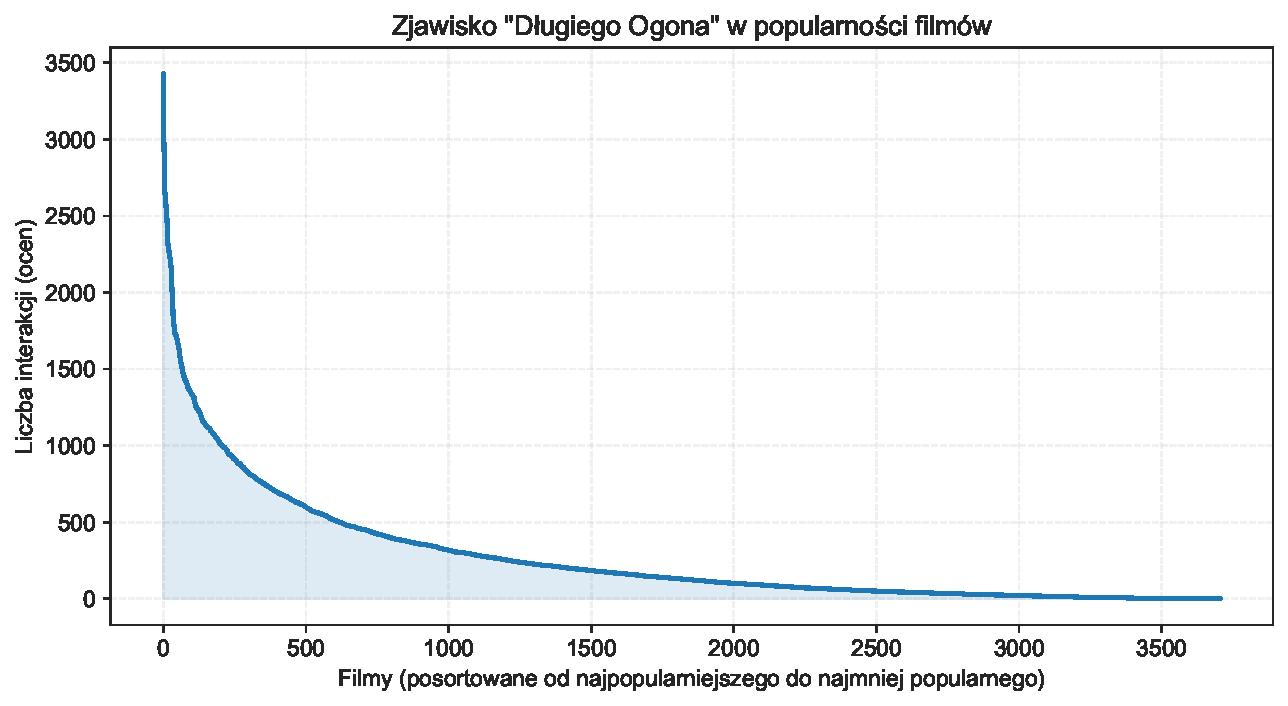
\includegraphics[width=0.85\textwidth]{img/movielens_long_tail.pdf}
    \caption{Rozkład popularności filmów w zbiorze MovieLens 1M przedstawiający zjawisko długiego ogona (\foreignlanguage{english}{\textit{Long-Tail Distribution}}).}
    \label{fig:long_tail}
    \vspace{1.5mm}

    {\raggedright \small \textbf{Źródło:} opracowanie własne.\par}
\end{figure}

Katalog filmowy dzieli się na dwie wyraźne strefy \footcite[100]{celmaMusicRecommendationDiscovery2010}:
\begin{itemize}
    \item \textbf{Głowę popytu (\foreignlanguage{english}{\textit{Head}}):} wąską grupę najpopularniejszych produkcji kinowych (tzw. hitów), które skupiają przeważającą część całkowitej liczby ocen w systemie. Tradycyjnie to ta część oferty była faworyzowana w erze analogowej ze względu na ograniczenia fizycznej przestrzeni sklepowej i wysokie koszty dystrybucji, które wymuszały na dystrybutorach selekcję wyłącznie pozycji o masowej popularności \footcite[14--15, 100]{celmaMusicRecommendationDiscovery2010}.
    \item \textbf{Długi ogon (\foreignlanguage{english}{\textit{Tail}}):} obszerną listę niszowych, mniej znanych lub starszych tytułów o niskiej częstotliwości odtworzeń. W dobie cyfrowej, po wyeliminowaniu fizycznych ograniczeń magazynowych i półkowych, cała ta niszowa oferta może pozostawać stale dostępna dla użytkowników, tworząc ogromną sumę małych rynków o bardzo wysokim potencjale zaspokajania specyficznych i zróżnicowanych gustów \footcite[100]{celmaMusicRecommendationDiscovery2010}.
\end{itemize}

Z biznesowego i funkcjonalnego punktu widzenia spersonalizowany system rekomendacyjny na rynku VOD musi potrafić trafnie proponować pozycje z długiego ogona, zapobiegając zjawisku monopolizacji uwagi widza wyłącznie przez najpopularniejsze hity \footcite[23]{checinskiSystemyRekomendacjiRemedium2023}. W dobie tzw. cyfrowej klęski urodzaju, gdy platformy streamingowe oferują tysiące filmów i seriali, użytkownicy stają w obliczu przeładowania informacyjnego, w którym samodzielne dotarcie do interesujących pozycji staje się wysoce utrudnione, a zapoznanie się z pełną ofertą katalogową jest fizycznie niemożliwe \footcite[19]{checinskiSystemyRekomendacjiRemedium2023}. Brak skutecznego mechanizmu personalizacji sprawia, że uwaga użytkowników koncentruje się wyłącznie na tytułach najgłośniejszych i powszechnie promowanych, co prowadzi do marnowania potencjału niszowej części biblioteki serwisu \footcite[19]{checinskiSystemyRekomendacjiRemedium2023}. Wdrożenie algorytmów zdolnych do eksploracji długiego ogona i kierowania uwagi widzów z obszaru głowy popytu ku pozycjom niszowym pozwala na pełniejsze wykorzystanie zasobów, zwiększa satysfakcję i lojalność odbiorców oraz maksymalizuje zaangażowanie w korzystanie z platformy \footcite[14--15, 23]{celmaMusicRecommendationDiscovery2010, checinskiSystemyRekomendacjiRemedium2023}.

Oryginalny zbiór MovieLens zawiera oceny jawne (\foreignlanguage{english}{\textit{explicit feedback}}) wyrażone w 5-stopniowej skali dyskretnej (od 1 do 5 gwiazdek). Choć oceny te dostarczają bardzo precyzyjnej i jednoznacznej informacji o stopniu satysfakcji użytkownika, w rzeczywistych systemach rekomendacyjnych współczesnych platform wideo występują one niezwykle rzadko. Wynika to z faktu, że czynność ta nakłada na odbiorcę dodatkowe obciążenie poznawcze i wymaga intencjonalnego działania po seansie, co zakłóca naturalną, bezwysiłkową konsumpcję treści --- większość widzów chce po prostu oglądać kolejne materiały, a nie dokonywać ich ewaluacji \footcite[452]{rendleBPRBayesianPersonalized2009}.

W konsekwencji głównym źródłem informacji dla algorytmów stają się ślady cyfrowe i interakcje dorozumiane (\foreignlanguage{english}{\textit{implicit feedback}}), takie jak odtworzenie filmu, czas jego oglądania, kliknięcie w miniaturę czy historia wyszukiwania \footcite[2]{suSurveyCollaborativeFiltering2009, checinskiSystemyRekomendacjiRemedium2023}. Dane te są gromadzone przez platformy całkowicie pasywnie, bez wysiłku ze strony widza, co pozwala na budowę znacznie większych i bardziej aktualnych zbiorów uczących, choć są one trudniejsze w interpretacji z uwagi na brak bezpośredniej deklaracji zadowolenia \footcite[452--453]{rendleBPRBayesianPersonalized2009}. Rozkład ocen jawnych w analizowanym zbiorze zaprezentowano na Rysunku \ref{fig:ratings_distribution}.

\begin{figure}[H]
    \centering
    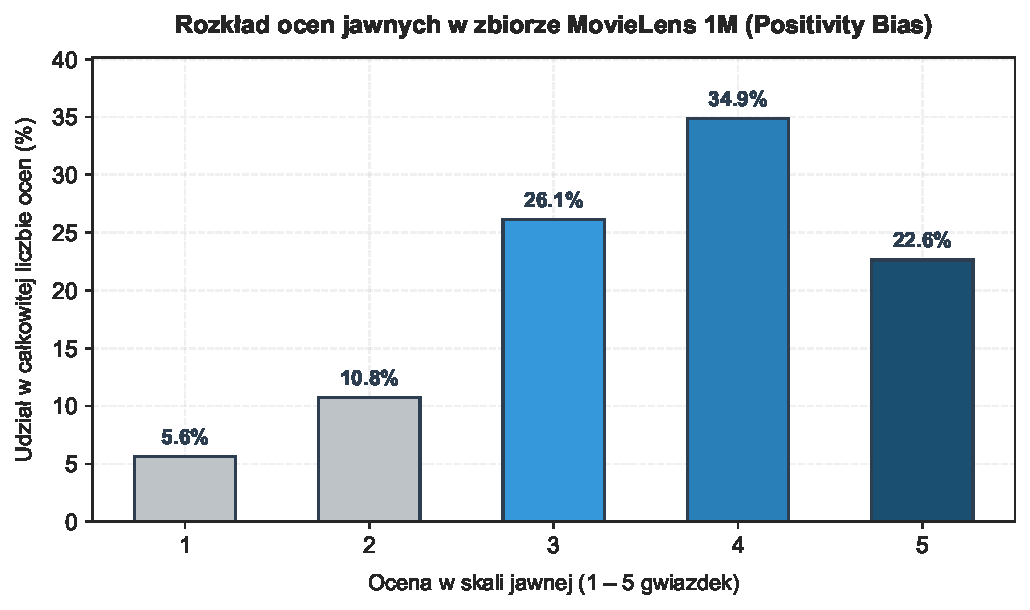
\includegraphics[width=0.82\linewidth]{img/movielens_ratings_distribution.pdf}
    \caption{Rozkład ocen jawnych w zbiorze MovieLens 1M obrazujący efekt zjawiska \foreignlanguage{english}{\textit{positivity bias}}}
    \label{fig:ratings_distribution}
    {\raggedright \small \textbf{Źródło:} opracowanie własne na podstawie danych z zestawu MovieLens 1M.\par}
\end{figure}

Analiza histogramu wykazuje silne skrzywienie pozytywne (\foreignlanguage{english}{\textit{positivity bias}}) -- użytkownicy znacznie chętniej oceniają filmy, które im się podobały, podczas gdy produkcje ocenione negatywnie są w logach niemal nieobecne (oceny 3, 4 i 5 stanowią ponad $80\%$ wszystkich wpisów). Zjawisko to jest bezpośrednią konsekwencją błędu selekcji; widzowie intuicyjnie wybierają do obejrzenia te tytuły, wobec których żywią już uprzednie pozytywne oczekiwania (np. ze względu na ulubiony gatunek czy obsadę), co wtórnie drastycznie ogranicza szansę na wystawienie niskiej noty \footcite[28]{celmaMusicRecommendationDiscovery2010}. W rezultacie obserwowany zbiór ocen jawnych nie odzwierciedla reprezentatywnego profilu gustu użytkownika wobec całego katalogu, a jedynie wobec jego wyselekcjonowanego ułamka \footcite[28]{celmaMusicRecommendationDiscovery2010}.

Zgodnie z metodologią zaproponowaną przez He i in. \footcite[7]{heNeuralCollaborativeFilteringKwiecien032017}, w celu dostosowania danych do realiów platform streamingowych dokonuje się przekształcenia binarnego oryginalnej macierzy ocen w macierz interakcji dorozumianych, oznaczaną jako $\mathbf{Y} \in \mathbb{R}^{M \times N}$ (gdzie $M = |\mathcal{U}|$ oznacza liczbę użytkowników, a $N = |\mathcal{I}|$ liczbę filmów). Zabieg ten pozwala na przekształcenie subiektywnego problemu regresji ocen w zadanie klasyfikacji binarnej (rekomendacji góry listy), co znacznie lepiej oddaje rzeczywiste zachowanie i procesy decyzyjne użytkowników w serwisach OTT, gdzie kluczowym wyborem jest decyzja o kliknięciu i rozpoczęciu odtwarzania danego tytułu \footcite[7]{heNeuralCollaborativeFilteringKwiecien032017}.

Przed przedstawieniem reguły dyskryminacyjnej zdefiniujmy elementy składowe wzoru:
\begin{itemize}
    \item $y_{ui}$ --- wartość wskaźnikowa określająca obecność zaobserwowanej relacji pomiędzy użytkownikiem $u \in \mathcal{U}$ a obiektem $i \in \mathcal{I}$,
    \item $y_{ui} = 1$ --- stan dodatni, oznaczający zarejestrowanie interakcji (np. wystawienie jakiejkolwiek oceny lub obejrzenie filmu),
    \item $y_{ui} = 0$ --- stan nieobserwowany, oznaczający brak zarejestrowanej akcji w logach systemowych.
\end{itemize}

Sformułowanie matematyczne funkcji binarnej przyjmuje postać:
\begin{equation}
    y_{ui} = \begin{cases} 1, & \text{jeśli zaobserwowano interakcję (użytkownik } u \text{ ocenił/obejrzał film } i\text{)} \\ 0, & \text{w przeciwnym razie (brak obserwacji)} \end{cases}
\end{equation}

Warto podkreślić, że wartość $y_{ui} = 0$ ma charakter wysoce niejednoznaczny semantycznie. Nie oznacza ona bowiem jawnej niechęci użytkownika do danego tytułu, lecz jedynie brak wiedzy o wchodzeniu w interakcję \footcite[2]{heNeuralCollaborativeFilteringKwiecien032017}. Użytkownik mógł nie obejrzeć filmu z powodów zupełnie niezależnych od jego gustu: mógł go nie zauważyć w katalogu, nie zostać na niego wyeksponowany przez interfejs platformy, bądź po prostu jeszcze na niego nie trafić \footcite[2]{heNeuralCollaborativeFilteringKwiecien032017, rendleBPRBayesianPersonalized2009}. Struktura ta stanowi fundamentalne wyzwanie w uczeniu maszynowym, gdyż zbiór danych nieobserwowanych ($y_{ui} = 0$) de facto reprezentuje jednocześnie rzeczywiste negatywne preferencje (użytkownik zna film, ale nie chce go obejrzeć), jak i potencjalne przyszłe interakcje dodatnie (użytkownik chętnie obejrzałby film, gdyby tylko dowiedział się o jego istnieniu), które model powinien poprawnie zidentyfikować i wybić na górę listy rekomendacji \footcite[453]{rendleBPRBayesianPersonalized2009}.


Rozkład aktywności użytkowników wykazuje duże zróżnicowanie -- od profilów okazjonalnych po użytkowników o skrajnie wysokiej liczbie obejrzanych pozycji. Aby wyeliminować zaburzenia wynikające ze skrajnie rzadkich profilów oraz pozycji znikających z katalogu bez historii ocen, zastosowano procedurę filtrowania typu $k$-\foreignlanguage{english}{\textit{core}} ($k = 5$) \footcite[7, sekcja 4.1.1]{heNeuralCollaborativeFilteringKwiecien032017}. Odrzucono wszystkich użytkowników oraz filmy posiadające mniej niż 5 zarejestrowanych interakcji. Operacja ta zapobiega występowaniu niemożliwych do wyuczenia trywialnych wektorów zerowych w warstwach embeddingów oraz stabilizuje proces wyznaczania normalizacji macierzy sąsiedztwa grafu dwudzielnego w modelach GNN \footcite[6, sekcja 2.1.1]{zhaoRecBoleUnifiedComprehensive2020}.

W celu zapewnienia ścisłej reprodukowalności eksperymentów i eliminacji błędów implementacyjnych, oczyszczone zbiory danych przekonwertowano do formatu Plików Atomowych (ang. \foreignlanguage{english}{\textit{Atomic Files}}) z rozszerzeniem \texttt{.inter}, stanowiącego standard wejściowy biblioteki RecBole \footcite[6, sekcja 2.1.2]{zhaoRecBoleUnifiedComprehensive2020}. Plik \texttt{.inter} przechowuje relacje w strukturze tabularycznej ze zdefiniowanymi typami pól \footcite[6, Tabela 3]{zhaoRecBoleUnifiedComprehensive2020}:
\begin{itemize}
    \item \texttt{user\_id:token} -- unikalny identyfikator użytkownika (sekwencja dyskretna),
    \item \texttt{item\_id:token} -- unikalny identyfikator filmu (sekwencja dyskretna),
    \item \texttt{rating:float} -- oryginalna ocena użytkownika (wykorzystywana pomocniczo),
    \item \texttt{timestamp:float} -- znacznik czasu interakcji.
\end{itemize}


Ewaluację modeli przeprowadzono w oparciu o proporcjonalny losowy podział danych (\foreignlanguage{english}{\textit{Ratio Splitting}}) w stosunku $80\% : 10\% : 10\%$ (odpowiednio: zbiór treningowy, walidacyjny i testowy), co stanowi standardowy protokół podziału danych typu \foreignlanguage{english}{\textit{ratio-based splitting}} obsługiwany przez bibliotekę RecBole \footcite[6, sekcja 2.1.1 oraz s. 7, sekcja 2.3.4]{zhaoRecBoleUnifiedComprehensive2020}.

Do trenowania modeli punktowych i parowych (Log Loss w NCF oraz BPR Loss w SVD/LightGCN) zastosowano procedurę próbkowania negatywnego (\foreignlanguage{english}{\textit{negative sampling}}). Dla każdej dodatniej pary $(u, i) \in \mathcal{E}$ losowano jednostajnie ze zbioru pozycji nieobserwowanych zestaw próbek negatywnych $(u, j) \in \mathcal{E}^-$ (gdzie $y_{uj} = 0$), przy zachowaniu stosunku $1:4$ (4 próbki negatywne na 1 pozycję dodatnią), co stanowi optymalny kompromis między stabilnością gradientu a czasem obliczeń \footcite[7, sekcja 4.1.2]{heNeuralCollaborativeFilteringKwiecien032017}. Zastosowanie elastycznej liczby próbek negatywnych (w optymalnym przedziale od 3 do 6) pozwala modelom optymalizowanym punktową stratą logarytmicznej na znaczące przełamanie ograniczeń klasycznych strat parowych typu BPR, które z natury parują wyłącznie jedną próbkę negatywną z dodatnią \footcite[8, sekcja 4.3]{heNeuralCollaborativeFilteringKwiecien032017}.



\newpage
Tabela \ref{tab:movielens_stats} przedstawia zbiorcze zestawienie parametrów statystycznych przygotowanego zbioru danych MovieLens 1M po przeprowadzeniu potoku przetwarzania.

\begin{table}[H]
    \centering
    \small
    \setlength{\tabcolsep}{6pt}
    \caption{Podsumowanie statystyczne zbioru danych MovieLens 1M wykorzystanego w eksperymentach}
    \label{tab:movielens_stats}
    \begin{tabular}{|l|c|}
        \hline
        \textbf{Parametr statystyczny}             & \textbf{Wartość dla zbioru MovieLens 1M (\texttt{ml-1m})} \\ \hline
        Liczba użytkowników ($|\mathcal{U}|$)      & 6\,040                                                    \\ \hline
        Liczba filmów ($|\mathcal{I}|$)            & 3\,706                                                    \\ \hline
        Liczba interakcji ($|\mathcal{E}|$)        & 1\,000\,209                                                \\ \hline
        Średnia liczba ocen na użytkownika         & 165{,}60                                                  \\ \hline
        Gęstość macierzy (\textit{Density})         & 4{,}47\%                                                  \\ \hline
        Rzadkość macierzy (\textit{Sparsity})       & 95{,}53\%                                                 \\ \hline
        Typ informacji zwrotnej                    & Interakcje dorozumiane (\textit{Implicit Feedback})       \\ \hline
    \end{tabular}
    \vspace{1.5mm}

    {\raggedright \small \textbf{Źródło:} opracowanie własne na podstawie danych MovieLens 1M.\par}
\end{table}

\subsection{Algorytmy filtrowania kolaboracyjnego}
\subsection{Algorytmy uczenia głębokiego}
\subsection{Algorytmy grafowych sieci neuronowych}
\subsection{Metryki oceny}
% !TEX root = ../PRACA_MAIN.tex
\section{Porównanie algorytmów rekomendacyjnych}

W niniejszym rozdziale przeprowadzono ewaluację i porównanie skuteczności wybranych algorytmów rekomendacyjnych. Głównym celem badań było zestawienie ze sobą modeli reprezentujących trzy różne paradygmaty: klasyczną faktoryzację macierzy (BPR), głębokie sieci neuronowe (NCF) oraz grafowe sieci neuronowe (LightGCN).

Rozdział został podzielony na trzy główne sekcje. W pierwszej z nich szczegółowo opisano proces doboru i optymalizacji hiperparametrów, mający na celu maksymalizację zdolności predykcyjnych każdego z modeli. W kolejnej części zestawiono wyniki eksperymentów przeprowadzonych na zbiorze danych MovieLens i poddano je analizie pod kątem przyjętych metryk oceny (m.in. NDCG oraz Recall). Rozdział kończy dyskusja uzyskanych wyników oraz wnioski dotyczące skuteczności i ograniczeń badanych architektur w zadaniu rekomendacji Top-N.

\subsection{Proces strojenia hiperparametrów}

W celu uzyskania stosunkowo najlepszych możliwych wyników badanie poprzedzono procesem doboru odpowiednich hiperparametrów. Przyjęto następującą metodologię. W pierwszej kolejności zbadano poziom wrażliwości algorytmów na zmiany wartości określonych parametrów. Następnie bazując na wynikach zdefiniowano okrojoną siatkę hiperparametrów dla każdej z metod i przy pomocy metody Grid Search polegającej na zbadaniu wszystkich możliwych kombinacji określonych wcześniej wartości wyłoniono najlepsze zestawy parametrów będące podstawą późniejszej analizy porównawczej.

Dobór parametrów poddanych analizie wrażliwości wynikał z ich kluczowego wpływu na zdolności predykcyjne oraz charakterystyki architektonicznej każdego z badanych algorytmów:
\begin{itemize}
    \item W modelu \textbf{ItemKNN} wybrano rozmiar sąsiedztwa ($k$) oraz współczynnik wygładzania (ang. \foreignlanguage{english}{\textit{shrinkage}}). Parametr $k$ determinuje, na ilu najbardziej podobnych elementach bazuje predykcja, co jest kluczowe w filtrowaniu opartym na sąsiedztwie. Współczynnik wygładzania pozwala z kolei na redukcję szumu statystycznego przy obliczaniu podobieństwa dla rzadko ocenianych przedmiotów.
    \item Dla modelu \textbf{BPR} skupiono się na współczynniku uczenia (ang. \foreignlanguage{english}{\textit{learning rate}}) oraz rozmiarze wektora cech ukrytych (ang. \foreignlanguage{english}{\textit{embedding size}}). Współczynnik uczenia determinuje zbieżność optymalizacji. Z kolei złożoność faktoryzacji macierzy rośnie wraz z wymiarem przestrzeni latentnej, dlatego optymalizacja tego parametru jest kluczowa dla balansu pomiędzy niedouczeniem a przeuczeniem.
    \item W głębokim modelu \textbf{NeuMF} analizie poddano współczynnik uczenia oraz prawdopodobieństwo odrzucenia neuronów (ang. \foreignlanguage{english}{\textit{dropout probability}}). Głębokie sieci neuronowe są wysoce podatne na zapamiętywanie danych treningowych (ang. \foreignlanguage{english}{\textit{overfitting}}), dlatego właściwy dobór parametru dropout jest niezbędny do uzyskania dobrej zdolności do generalizacji.
    \item W przypadku grafowego modelu \textbf{LightGCN} wytypowano wagę regularyzacji (ang. \foreignlanguage{english}{\textit{regularization weight}}) oraz liczbę warstw propagacji (ang. \foreignlanguage{english}{\textit{number of layers}}). Regularyzacja L2 kontroluje wielkość wag wektorów zapobiegając nadmiernemu dopasowaniu, podczas gdy liczba warstw odpowiada za eksplorację sygnałów wyższego rzędu w grafie (np. odległości 2-skokowe).
\end{itemize}

\subsubsection{Analiza wrażliwości}

Poniżej przedstawiono graficzne zestawienie wpływu badanych hiperparametrów na metrykę NDCG@10 dla każdego z algorytmów.
W przypadku modelu ItemKNN (Rysunek \ref{fig:sweep_itemknn}) można zaobserwować, że zwiększanie liczby uwzględnianych sąsiadów ($k$) konsekwentnie poprawia wyniki metryki NDCG@10 aż do wartości $k=200$, po czym przyrost ten naturalnie zwalnia. Regularyzacja \textit{shrinkage} z kolei nie przynosi w tym przypadku znaczących korzyści na zbiorze MovieLens 100K -- najwyższy wynik odnotowano dla braku wygładzania (wartość 0.0), a dalsze zwiększanie tego parametru skutkuje delikatnym i marginalnym spadkiem trafności.

\begin{figure}[H]
    \centering
    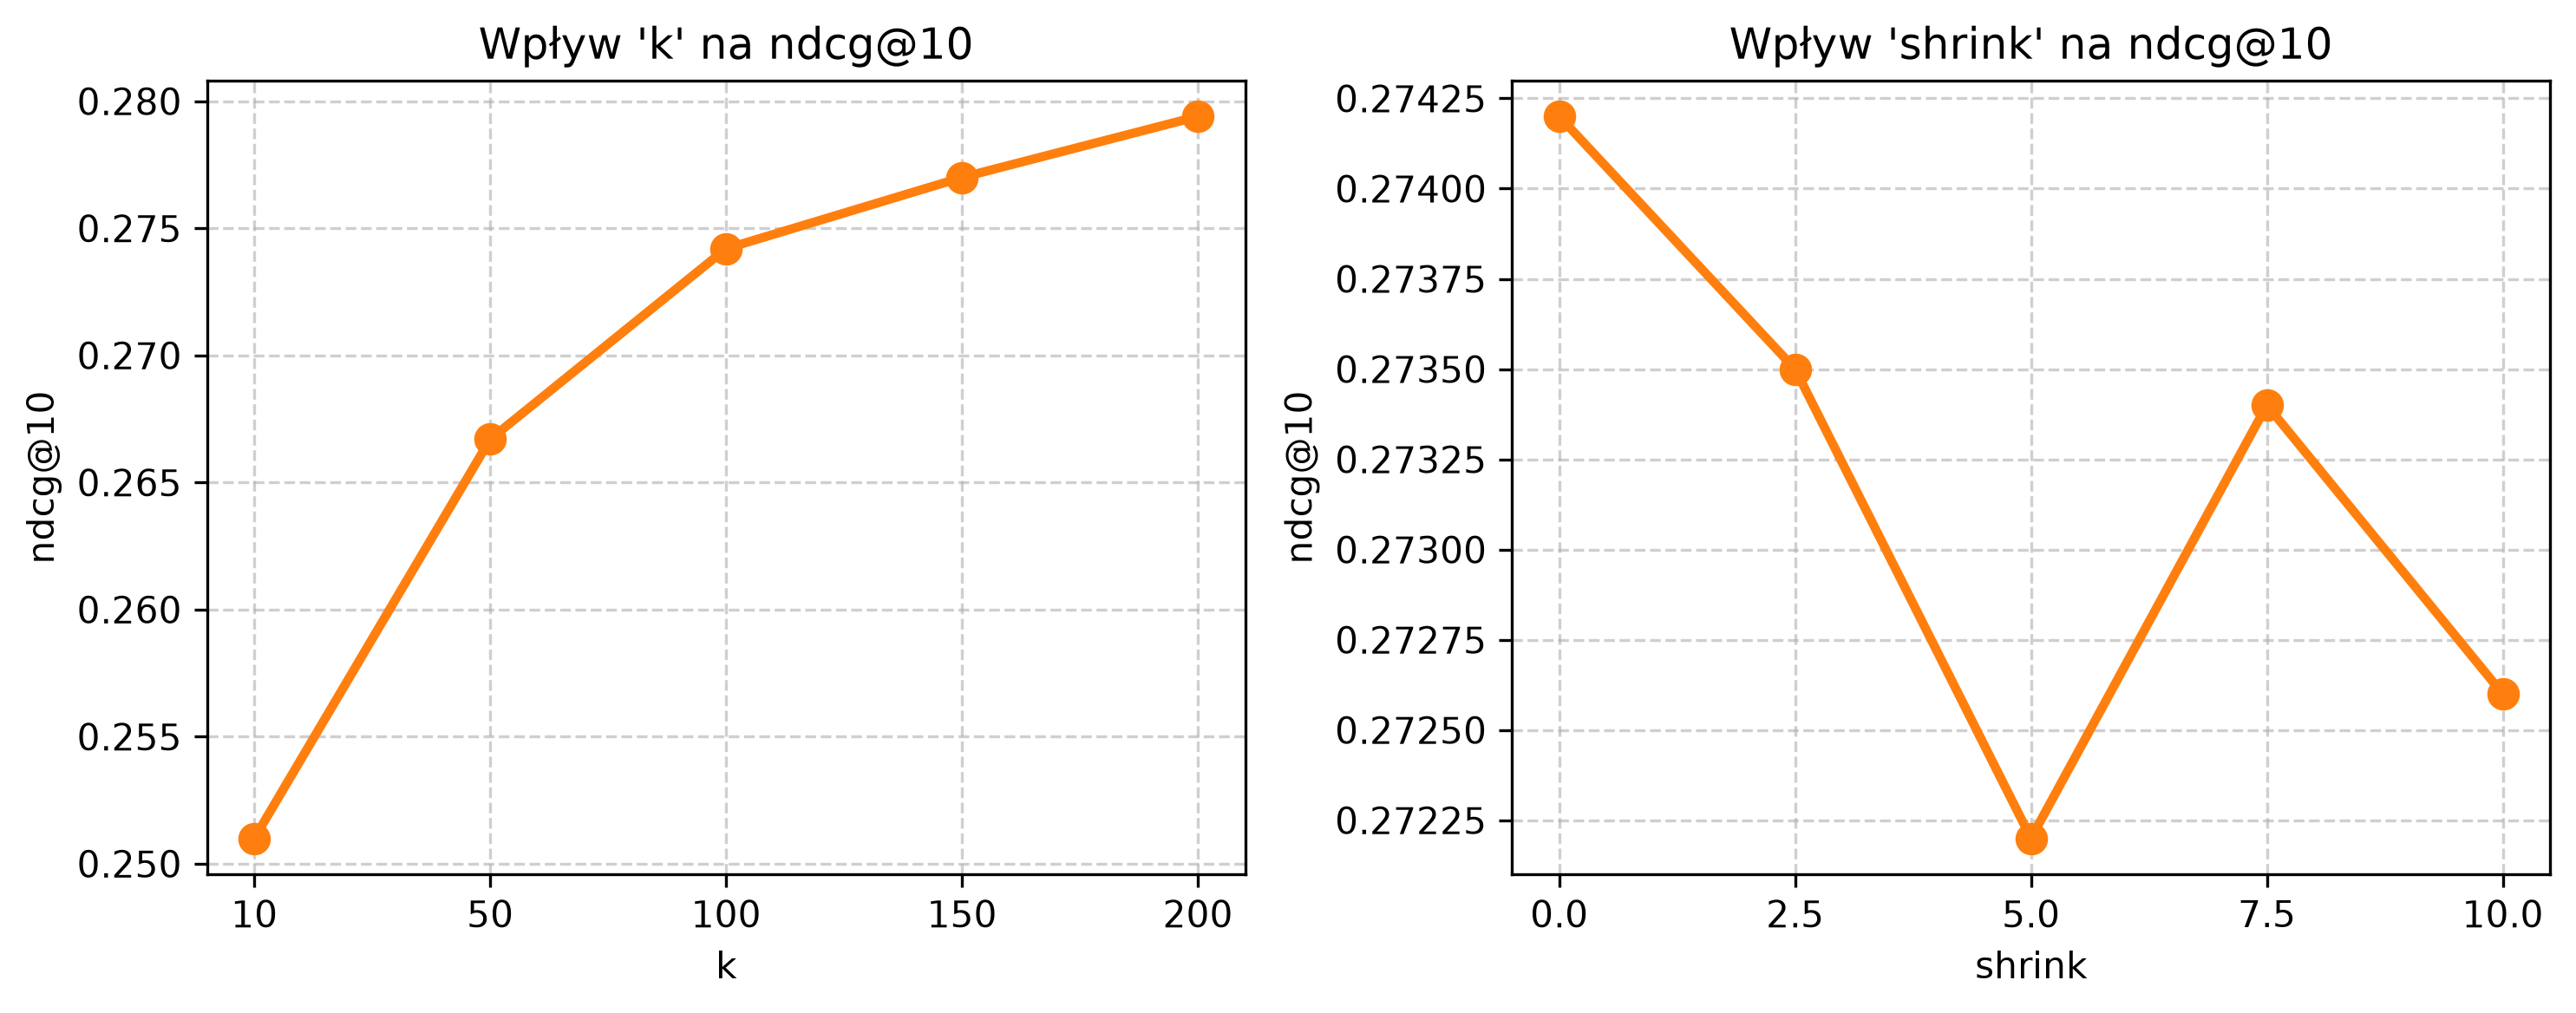
\includegraphics[width=\textwidth]{img/sweep_itemknn_summary.png}
    \caption{Wpływ hiperparametrów $k$ oraz \textit{shrinkage} na trafność modelu ItemKNN}
    \label{fig:sweep_itemknn}
    \vspace{0.2cm}\noindent{\raggedright \small \textbf{Źródło:} opracowanie własne.\par}
\end{figure}

Dla modelu faktoryzacji BPR (Rysunek \ref{fig:sweep_bpr}) analiza ujawnia klasyczną zależność optymalizacyjną. Współczynnik uczenia osiąga jednoznaczne optimum na poziomie 0.0005, zapewniając najwyższą trafność na poziomie NDCG@10 $\approx$ 0.2867. Większe wartości prowadzą do spadku trafności w wyniku niestabilności numerycznej. Z kolei rozmiar wektora cech wskazuje, że wartość 128 oferuje optymalną celność (niewielka przewaga nad 64), podczas gdy dalsze zwiększanie do wymiaru 256 skutkuje spadkiem skuteczności spowodowanym powolnym przeuczaniem się algorytmu na treningowej części zbioru.

\begin{figure}[H]
    \centering
    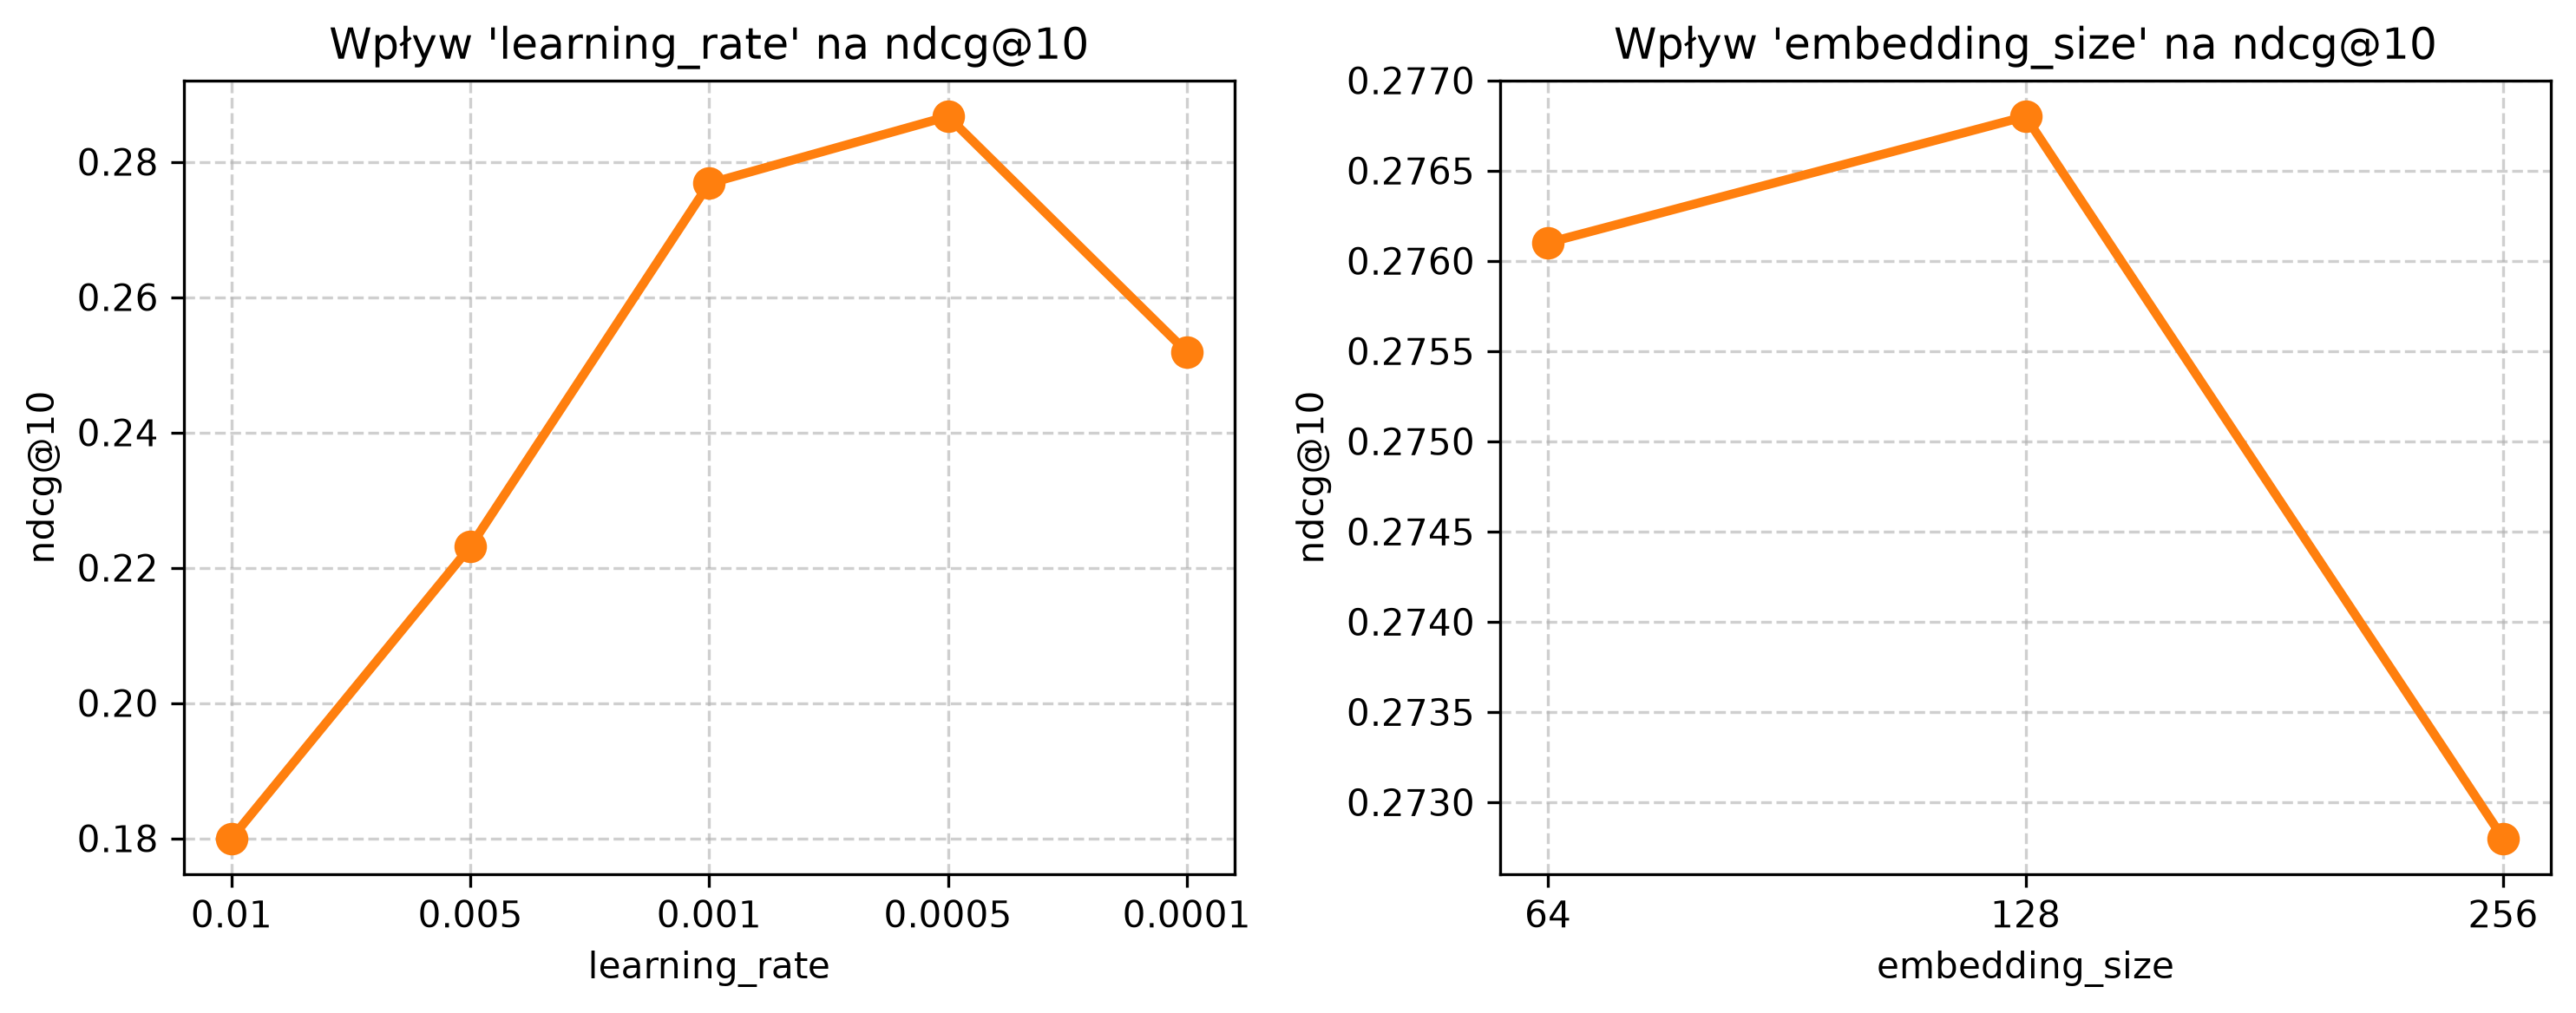
\includegraphics[width=\textwidth]{img/sweep_bpr_summary.png}
    \caption{Wpływ współczynnika uczenia oraz rozmiaru wektora zanurzeń na trafność modelu BPR}
    \label{fig:sweep_bpr}
    \vspace{0.2cm}\noindent{\raggedright \small \textbf{Źródło:} opracowanie własne.\par}
\end{figure}

Ocena parametrów hybrydowego modelu NeuMF (Rysunek \ref{fig:sweep_neumf}) potwierdza specyfikę głębokich sieci neuronowych. Widać jednoznacznie, że model zbiega do globalnego optimum przy \textit{learning rate} na poziomie 0.0001 (NDCG $\approx$ 0.2810). Parametr \textit{dropout} wykazuje z kolei wysoce czytelny punkt optymalny dla wartości 0.5. Pozwala to na odpowiednią, restrykcyjną regularyzację gęstych warstw, skutecznie hamując overfitting i zwiększając zdolność uogólniania wniosków.

\begin{figure}[H]
    \centering
    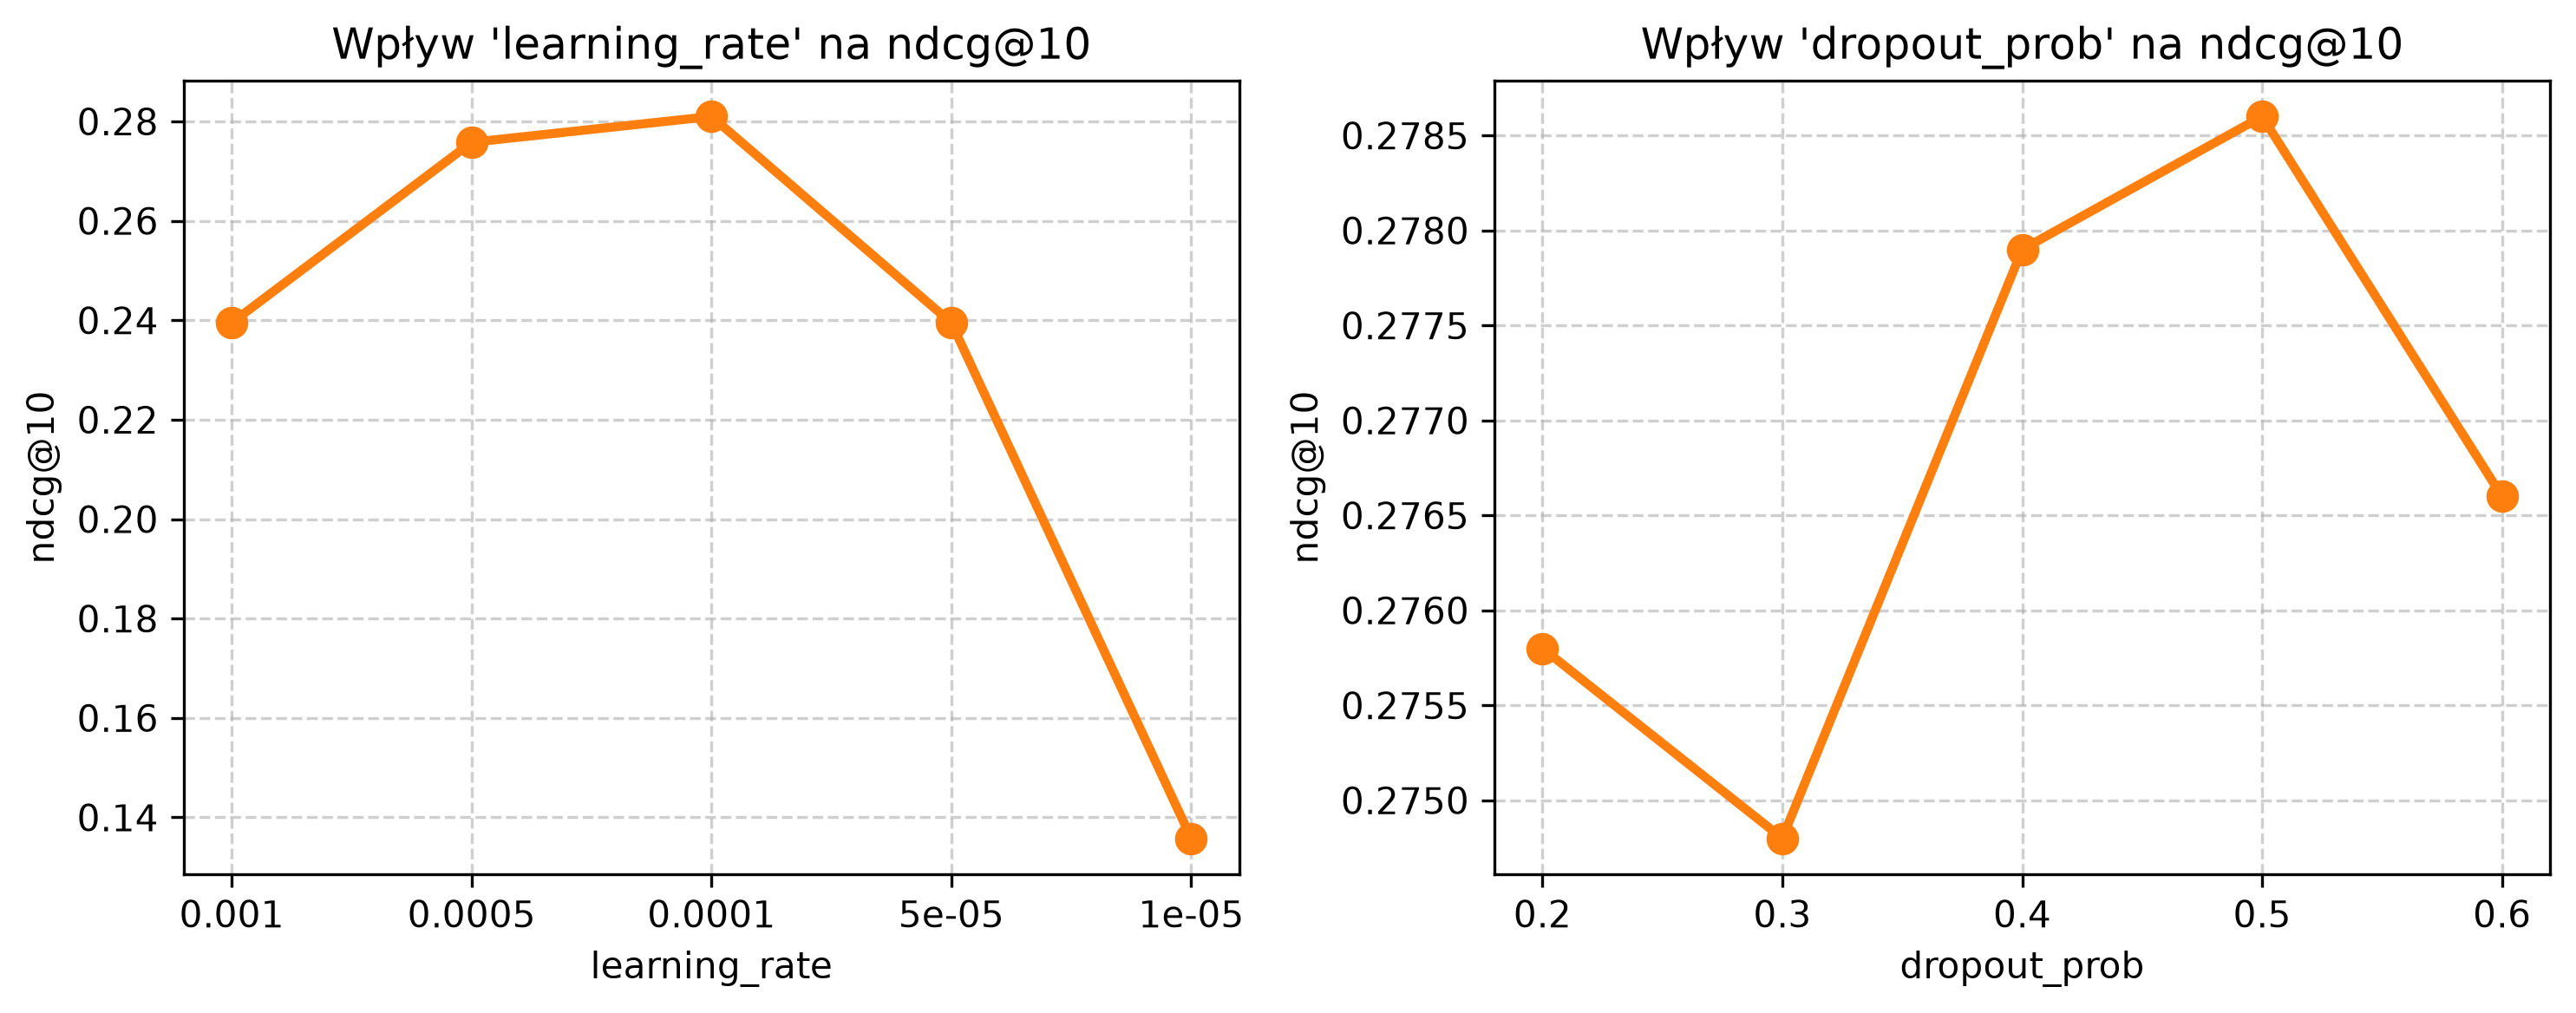
\includegraphics[width=\textwidth]{img/sweep_neumf_summary.png}
    \caption{Wpływ współczynnika uczenia oraz parametru dropout na trafność modelu NeuMF}
    \label{fig:sweep_neumf}
    \vspace{0.2cm}\noindent{\raggedright \small \textbf{Źródło:} opracowanie własne.\par}
\end{figure}

Ostatnim etapem analizy była ocena grafowego modelu LightGCN (Rysunek \ref{fig:sweep_lightgcn}). Architektura ta bazuje na propagacji informacji wzdłuż krawędzi, co ma swoje odzwierciedlenie na wykresie: zastosowanie dwóch warstw propagacji (\textit{n\_layers = 2}) okazało się optymalne. Zwiększanie liczby warstw do 3 lub 4 nieznacznie pogarsza wyniki, co jest klasycznym objawem problemu nadmiernego wygładzenia sygnałów (ang. \foreignlanguage{english}{\textit{over-smoothing}}). Zastosowanie odpowiedniej siły kary za wielkość wag również posiada ostry szczyt użyteczności: \textit{reg\_weight = 0.10} maksymalizuje końcową precyzję predykcji tego algorytmu.

\begin{figure}[H]
    \centering
    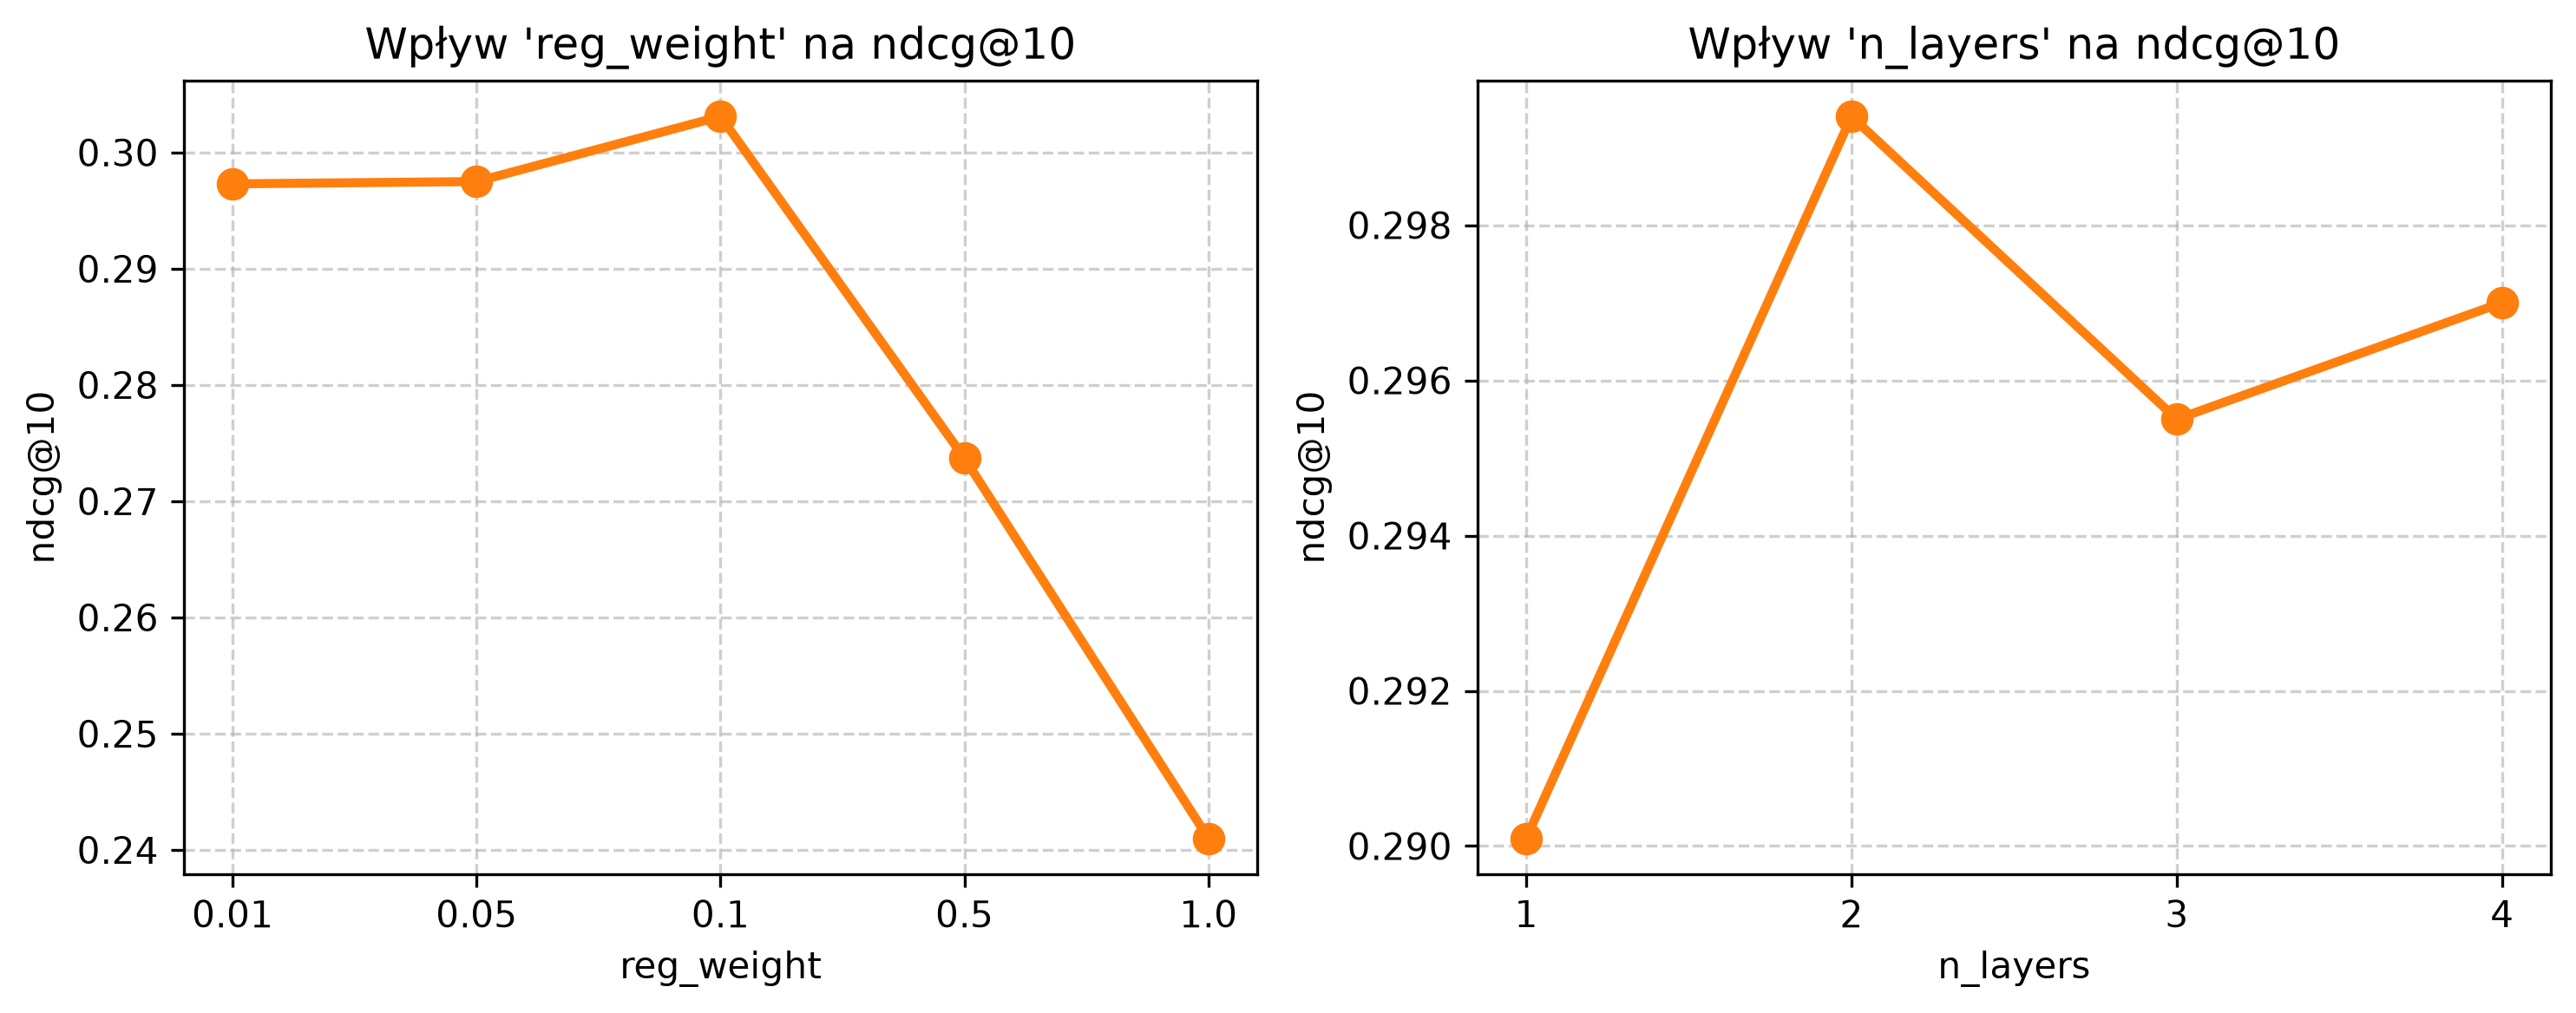
\includegraphics[width=\textwidth]{img/sweep_lightgcn_summary.png}
    \caption{Wpływ wagi regularyzacji oraz liczby warstw propagacji na trafność modelu LightGCN}
    \label{fig:sweep_lightgcn}
    \vspace{0.2cm}\noindent{\raggedright \small \textbf{Źródło:} opracowanie własne.\par}
\end{figure}


\subsubsection{Przeszukiwanie siatki parametrów --- Grid Search}

Do ostatecznej optymalizacji hiperparametrów wykorzystano metodę przeszukiwania siatki (\textit{Grid Search}). Jest to podejście deterministyczne, w którym dla każdego badanego parametru definiuje się dyskretny zbiór wartości, a następnie sprawdza każdą możliwą ich kombinację. Złożoność obliczeniowa tego procesu rośnie wykładniczo wraz z liczbą analizowanych wymiarów, co w naturalny sposób narzuca konieczność wcześniejszej redukcji przestrzeni wariantów.

Dzięki przeprowadzonej wcześniej, szczegółowej analizie wrażliwości (Sekcja 3.1.1) udało się odrzucić nieperspektywiczne przedziały wartości i drastycznie zawęzić ostateczną przestrzeń poszukiwań. Pozwoliło to na bezpieczne wykorzystanie metody \textit{Grid Search}, która w przeciwieństwie do podejść stochastycznych (takich jak \foreignlanguage{english}{\textit{Random Search}}) gwarantuje bezwzględne odnalezienie globalnego optimum w obrębie zadanej siatki. Opierając się na wytycznych z analizy, dla każdego algorytmu zdefiniowano okrojoną przestrzeń hiperparametrów, którą zestawiono w Tabeli \ref{tab:grid_search_space}. Zgodnie z metodologią badawczą, dla każdej możliwej konfiguracji zdefiniowanej w siatce inicjowano całkowicie niezależny proces uczenia od podstaw. Ewaluacja poszczególnych wariantów odbywała się wyłącznie na wyodrębnionym zbiorze walidacyjnym, co pozwalało na obiektywny wybór modelu i chroniło finalny zbiór testowy przed zjawiskiem przedwczesnego dopasowania. Za ostateczne kryterium wyboru najlepszego zestawu hiperparametrów przyjęto maksymalizację metryki NDCG@10.

Warto w tym miejscu zaznaczyć, że współczesne algorytmy rekomendacyjne -- w szczególności te oparte na sieciach neuronowych -- charakteryzują się rozbudowaną przestrzenią konfiguracyjną. Jednoczesna optymalizacja wszystkich dostępnych hiperparametrów przy użyciu metody \textit{Grid Search} była niemożliwa ze względu na wykładniczy wzrost czasu trwania obliczeń. Z tego powodu proces strojenia świadomie ograniczono wyłącznie do kluczowych parametrów, zidentyfikowanych w analizie wrażliwości jako najbardziej wpływowe dla poszczególnych architektur.

Zdecydowana większość pozostałych ustawień procesu uczenia, niewyszczególnionych w Tabeli \ref{tab:grid_search_space}, została ustandaryzowana i zachowana na stałym poziomie dla badanych algorytmów. Do aktualizacji wag wykorzystano optymalizator Adam, będący powszechnie uznanym standardem w środowisku RecBole. Rozmiar partii danych ustalono na 4096, co zapewniło odpowiednią stabilność numeryczną gradientu. Maksymalną liczbę iteracji ograniczono do 100 epok, z włączonym mechanizmem wczesnego zatrzymywania -- trening przerywano, gdy metryka NDCG@10 na zbiorze walidacyjnym nie uległa poprawie przez 10 kolejnych epok. Strategię negatywnego próbkowania uzależniono z kolei od specyfiki optymalizacji. Algorytmy bazujące na parowej funkcji straty BPR (klasyczny BPR oraz LightGCN) trenowano w schemacie 1:1, parując każdą interakcję pozytywną z jedną losową interakcją negatywną. Z kolei model NeuMF, zoptymalizowany pod kątem straty punktowej, trenowano stosując proporcję 1:4 (cztery próbki negatywne na jedną obserwowaną). Odpowiednie dostosowanie tego aspektu do natywnych mechanizmów poszczególnych architektur gwarantuje, że końcowa ewaluacja w pełni oddaje ich faktyczny potencjał.

\begin{table}[H]
    \centering
    \caption{Zestawienie przestrzeni hiperparametrów (siatki) dla poszczególnych algorytmów}
    \label{tab:grid_search_space}
    \begin{tabular}{|l|l|l|}
    \hline
    \textbf{Model}            & \textbf{Parametr}        & \textbf{Przestrzeń poszukiwań (Grid)} \\ \hline
    \multirow{2}{*}{ItemKNN}  & $k$                      & \{100, 150, 200\}                     \\ \cline{2-3}
                              & \textit{shrink}          & \{0.0, 2.5, 5.0, 7.5, 10.0\}          \\ \hline
    \multirow{2}{*}{BPR}      & \textit{learning\_rate}  & \{0.001, 0.0005, 0.0001\}             \\ \cline{2-3}
                              & \textit{embedding\_size} & \{64, 128\}                           \\ \hline
    \multirow{2}{*}{NeuMF}    & \textit{learning\_rate}  & \{0.0005, 0.0001, 0.00005\}           \\ \cline{2-3}
                              & \textit{dropout\_prob}   & \{0.4, 0.5, 0.6\}                     \\ \hline
    \multirow{2}{*}{LightGCN} & \textit{reg\_weight}     & \{0.01, 0.05, 0.1\}                   \\ \cline{2-3}
                              & \textit{n\_layers}       & \{2, 4\}                              \\ \hline
\end{tabular}


    \vspace{0.2cm}\noindent{\raggedright \small \textbf{Źródło:} opracowanie własne.\par}
\end{table}

Wyniki procesu optymalizacji pozwoliły na wyłonienie ostatecznych architektur, które posłużą do finalnego porównania skuteczności algorytmów w kolejnym podrozdziale. Zestawienie wyselekcjonowanych parametrów przedstawiono w Tabeli \ref{tab:finalne_parametry}:
\begin{itemize}
    \item \textbf{ItemKNN}: Najlepszą celność uzyskano dla sąsiedztwa $k=100$ oraz wygładzania \textit{shrinkage} $= 7.5$ (NDCG@10 $= 0.2734$).
    \item \textbf{BPR}: Wariant z optymalizacją bayesowską najlepiej operował w przestrzeni latentnej o rozmiarze $128$ przy kroku uczenia równym $0.001$ (NDCG@10 $= 0.2837$).
    \item \textbf{NeuMF}: Algorytm oparty na głębokich sieciach neuronowych osiągnął globalne optimum dla współczynnika odrzucenia (dropout) rzędu $0.5$ oraz współczynnika uczenia $0.0005$ (NDCG@10 $= 0.2895$). Pozostałe, stałe parametry architektoniczne (w tym rozmiary warstw ukrytych) zostały zachowane na podstawie wcześniejszej analizy.
    \item \textbf{LightGCN}: Model grafowy zdominował zestawienie testowe, uzyskując najwyższą bezwzględną trafność (NDCG@10 $= 0.3021$) dla $2$ warstw propagacji wzdłuż krawędzi oraz wagi regularyzacji L2 na poziomie $0.1$.
\end{itemize}

Powyższe zestawy parametrów gwarantują, że podczas ostatecznej ewaluacji każdy z modeli będzie operował na możliwie najlepiej dobranych wartościach i osiągał optymalne wyniki.

\begin{table}[H]
    \centering
    \caption{Wyselekcjonowane, optymalne wartości hiperparametrów dla badanych modeli}
    \label{tab:finalne_parametry}
    \begin{tabular}{|l|l|c|}
    \hline
    \textbf{Model} & \textbf{Parametr} & \textbf{Optymalna wartość} \\ \hline
    \multirow{2}{*}{ItemKNN}  & $k$ & 100 \\ \cline{2-3}
                              & \textit{shrink} & 7.5 \\ \hline
    \multirow{2}{*}{BPR}      & \textit{learning\_rate} & 0.001 \\ \cline{2-3}
                              & \textit{embedding\_size} & 128 \\ \hline
    \multirow{2}{*}{NeuMF}    & \textit{learning\_rate} & 0.0005 \\ \cline{2-3}
                              & \textit{dropout\_prob} & 0.5 \\ \hline
    \multirow{2}{*}{LightGCN} & \textit{reg\_weight} & 0.1 \\ \cline{2-3}
                              & \textit{n\_layers} & 2 \\ \hline
\end{tabular}


    \vspace{0.2cm}\noindent{\raggedright \small \textbf{Źródło:} opracowanie własne.\par}
\end{table}

\subsection{Wyniki badań}

W niniejszym podrozdziale zaprezentowano ostateczne zestawienie skuteczności badanych algorytmów. Ocenę przeprowadzono na odseparowanym zbiorze testowym, gwarantując tym samym obiektywną miarę zdolności modeli do generalizacji. Zgodnie z wcześniej przyjętą metodologią, predykcje poszczególnych architektur oceniono z wykorzystaniem metryk NDCG@10, Recall@10, HR@10 oraz MRR@10. Pełne zestawienie wyników zaprezentowano w Tabeli \ref{tab:wyniki_eksperymentow}.

\begin{table}[H]
    \centering
    \caption{Porównanie wyników metryk oceny dla testowanych algorytmów rekomendacyjnych na zbiorze MovieLens 100K.}
    \label{tab:wyniki_eksperymentow}
    \begin{tabular}{|l|c|c|c|c|}
\hline
\textbf{Model} & \textbf{NDCG@10} & \textbf{Recall@10} & \textbf{Hit@10} & \textbf{MRR@10} \\ \hline
ItemKNN & 0.2734 & 0.2336 & 0.7497 & 0.4392 \\ \hline
BPR & 0.2837 & \underline{0.2437} & 0.7603 & 0.4525 \\ \hline
NeuMF & \underline{0.2895} & 0.2435 & \textbf{0.7720} & \underline{0.4744} \\ \hline
LightGCN & \textbf{0.3021} & \textbf{0.2529} & \underline{0.7678} & \textbf{0.4835} \\ \hline
\end{tabular}

    \vspace{0.2cm}\noindent{\raggedright \small \textbf{Źródło:} opracowanie własne.\par}
\end{table}

Analiza powyższej tabeli pozwala na wyciągnięcie kilku kluczowych wniosków, które wpisują się w historyczną ewolucję systemów rekomendacyjnych. Punktem odniesienia w eksperymencie był najprostszy algorytm oparty na sąsiedztwie -- ItemKNN, który uzyskał najniższe, bazowe wyniki. Wprowadzenie klasycznej faktoryzacji macierzy (BPR) znacząco poprawiło jakość rekomendacji (wzrost NDCG z 0.2734 na 0.2837), co dowodzi wyższości uczenia się cech ukrytych nad prostymi heurystykami podobieństwa.

Wykorzystanie głębokich sieci neuronowych w modelu NeuMF przyniosło dalszą poprawę w większości metryk, jednak na szczególną uwagę zasługuje relacja między wskaźnikami HR@10 a NDCG@10. Choć NeuMF wygrał w kategorii HR@10 (0.7720), co oznacza, że skuteczniej umieszczał przynajmniej jeden trafny element w pierwszej dziesiątce, to ustąpił w rankingu NDCG. Dowodzi to, że osiągający najwyższe wyniki w zestawieniu grafowy model LightGCN znacznie lepiej radzi sobie z precyzyjnym pozycjonowaniem trafnych rekomendacji na samym szczycie listy. Architektura grafowa, dzięki jawnej propagacji sygnałów między użytkownikami a przedmiotami, uzyskała najwyższe wartości NDCG@10 (0.3021) oraz MRR@10 (0.4835).

\subsubsection{Krzywe zbieżności i stabilność procesu uczenia}

Zestawienie końcowych wyników uzupełniono o analizę dynamiki procesu uczenia poszczególnych architektur. Na Rysunku \ref{fig:learning_curves} zaprezentowano krzywe zbieżności (ang. \foreignlanguage{english}{\textit{learning curves}}) rejestrujące zmianę metryki NDCG@10 na zbiorze walidacyjnym w trakcie trwania optymalizacji, aż do momentu aktywacji mechanizmu wczesnego zatrzymywania.

\begin{figure}[H]
    \centering
    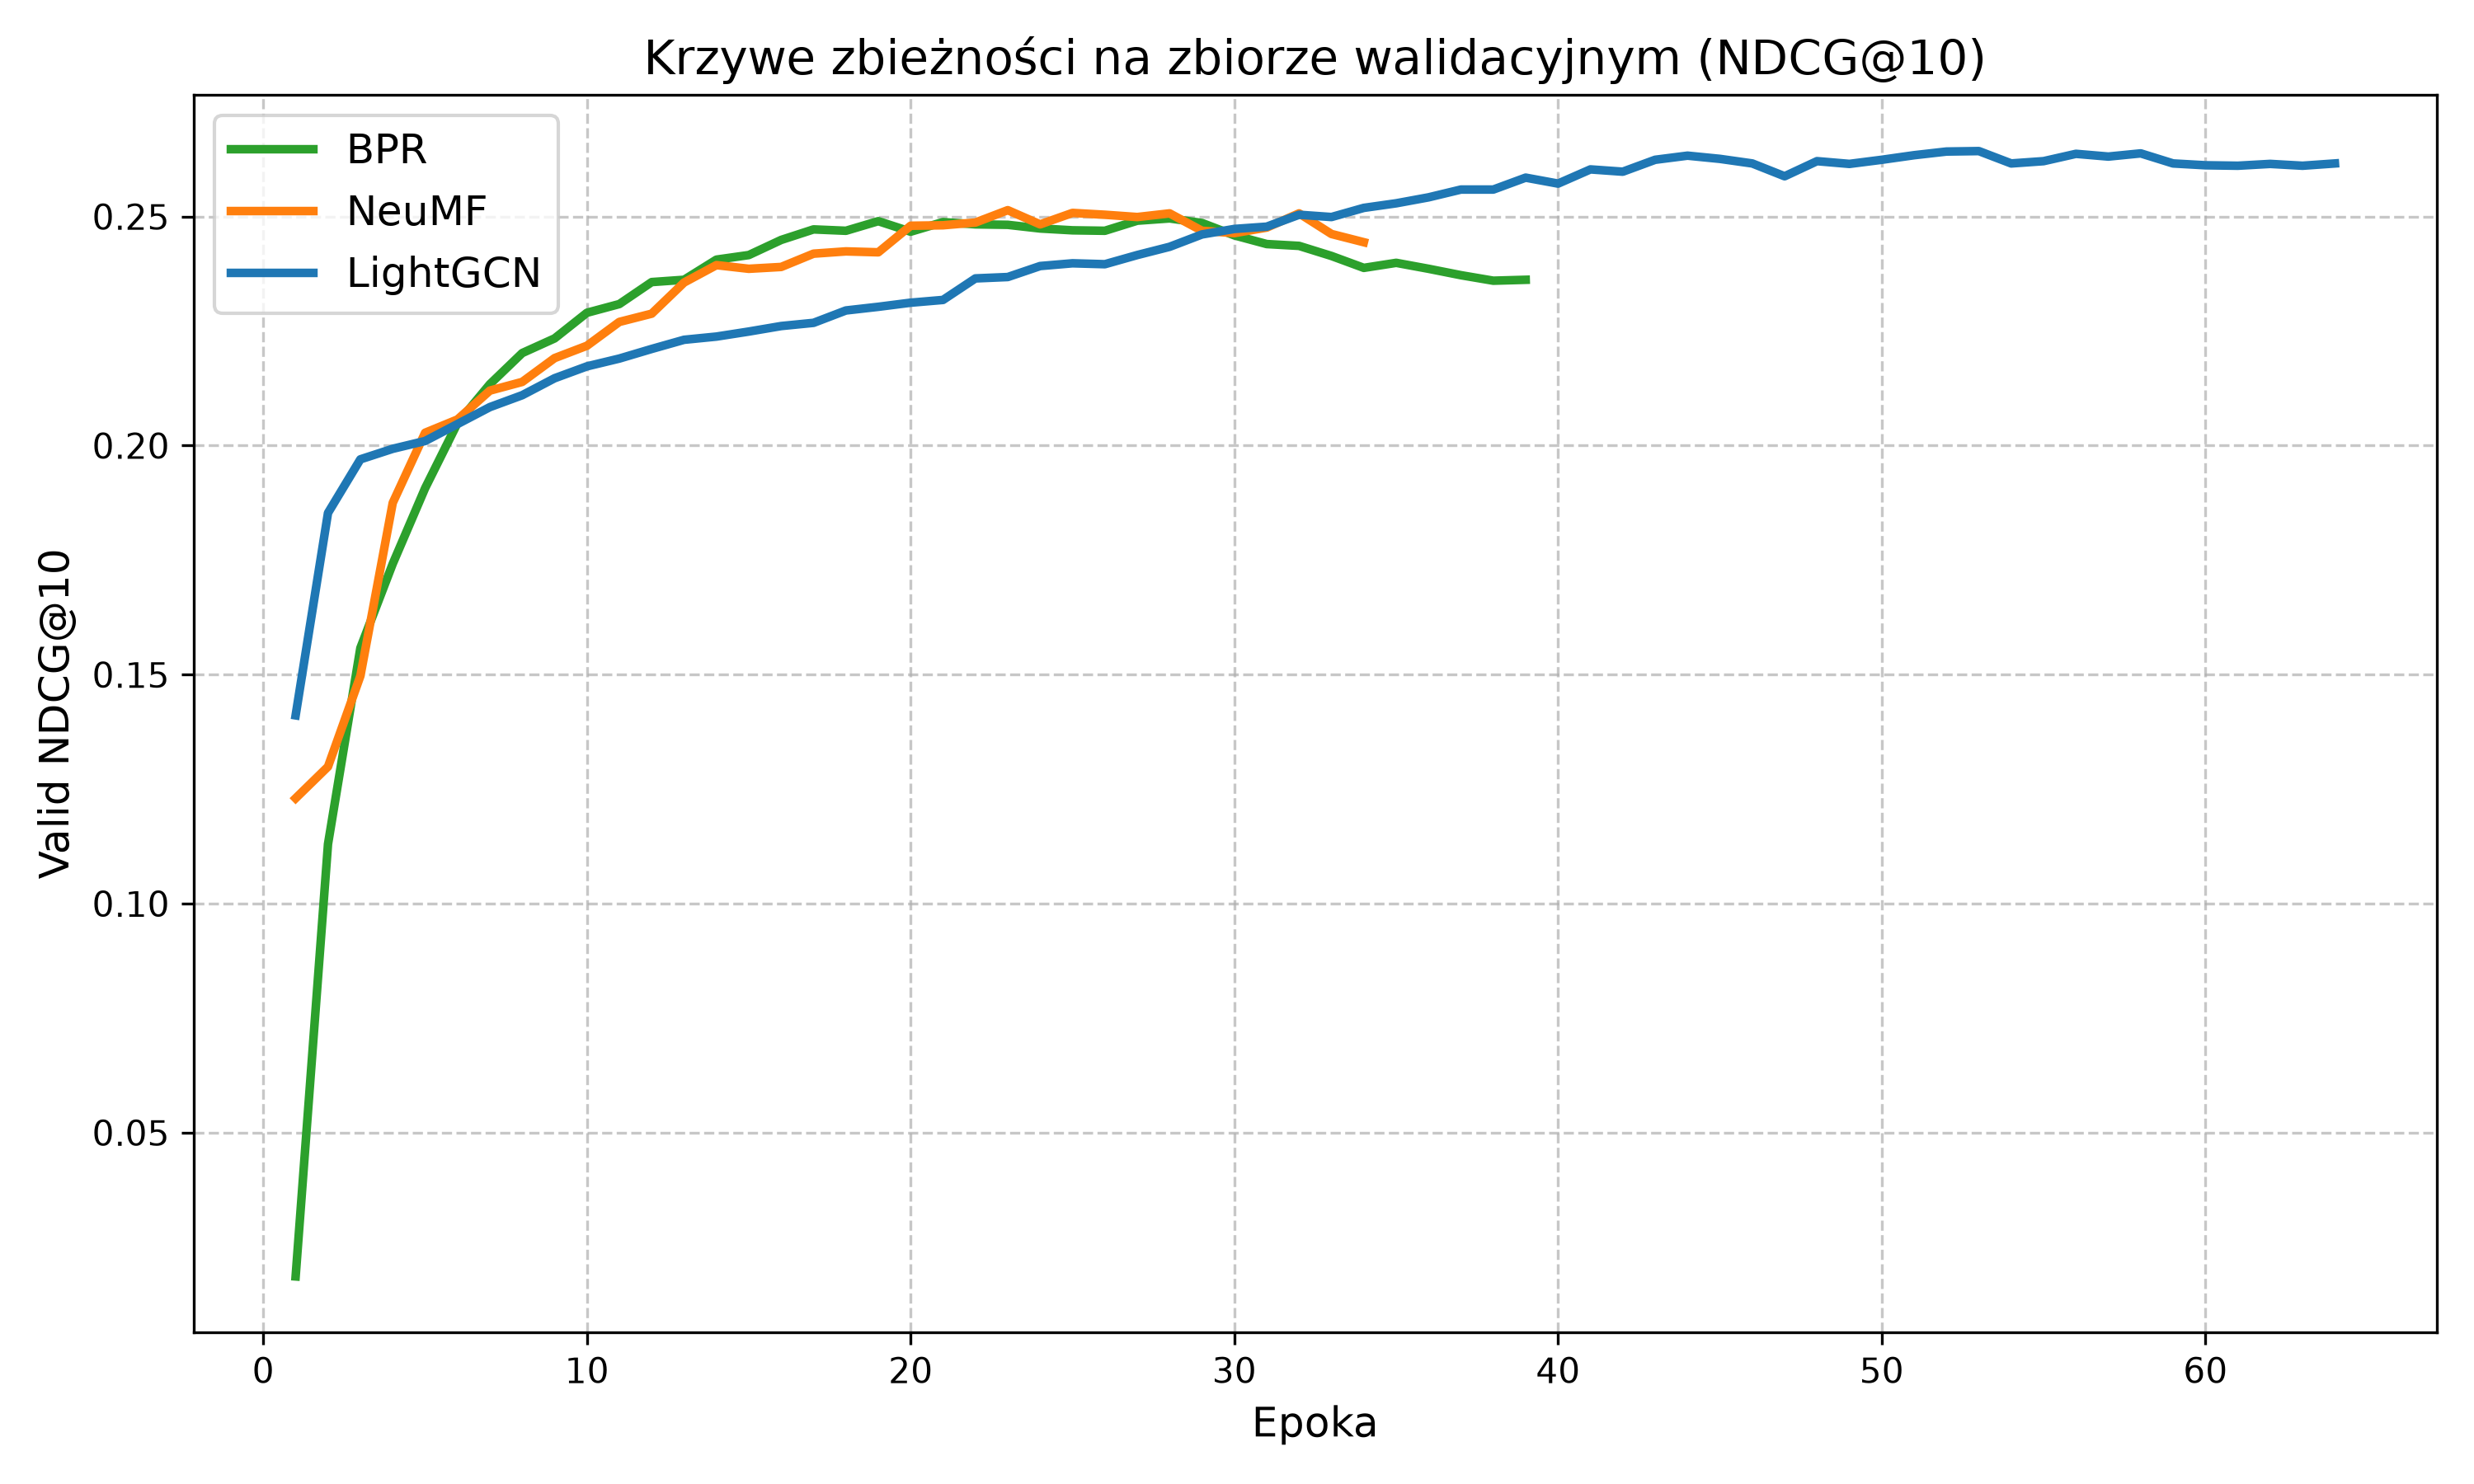
\includegraphics[width=0.85\textwidth]{img/learning_curves.png}
    \caption{Krzywe zbieżności metryki NDCG@10 na zbiorze walidacyjnym dla algorytmów BPR, NeuMF oraz LightGCN.}
    \label{fig:learning_curves}
    \vspace{0.2cm}\noindent{\raggedright \small \textbf{Źródło:} opracowanie własne.\par}
\end{figure}

Analiza krzywych ujawnia interesujące różnice w sposobie optymalizacji. Klasyczny model faktoryzacji macierzy (BPR) wykazuje najszybsze tempo zbieżności -- jego trafność gwałtownie rośnie już w pierwszych iteracjach, osiągając lokalne optimum w okolicach 20. epoki. Następnie można zaobserwować delikatny spadek jakości, co świadczy o podatności na przeuczenie na zbiorze treningowym. Z kolei model grafowy (LightGCN) startuje z niższego poziomu i uczy się znacznie wolniej, jednak jego krzywa jest wysoce stabilna. Ostatecznie, proces powolnego propagowania sygnałów w grafie pozwala na przekroczenie pułapu wyznaczonego przez BPR i NeuMF, a optymalna zbieżność osiągana jest znacznie później.

\subsubsection{Koszty obliczeniowe a skuteczność algorytmów}

Ostatnim elementem ewaluacji jest analiza relacji nakładów obliczeniowych (czasu optymalizacji modelu) do uzyskiwanej trafności predykcji. Jest to kluczowy wskaźnik inżynieryjny w środowiskach produkcyjnych, w których systemy rekomendacyjne muszą być regularnie i szybko dotrenowywane nowymi danymi. Zależność tę zilustrowano na Rysunku \ref{fig:time_vs_ndcg}.

\begin{figure}[H]
    \centering
    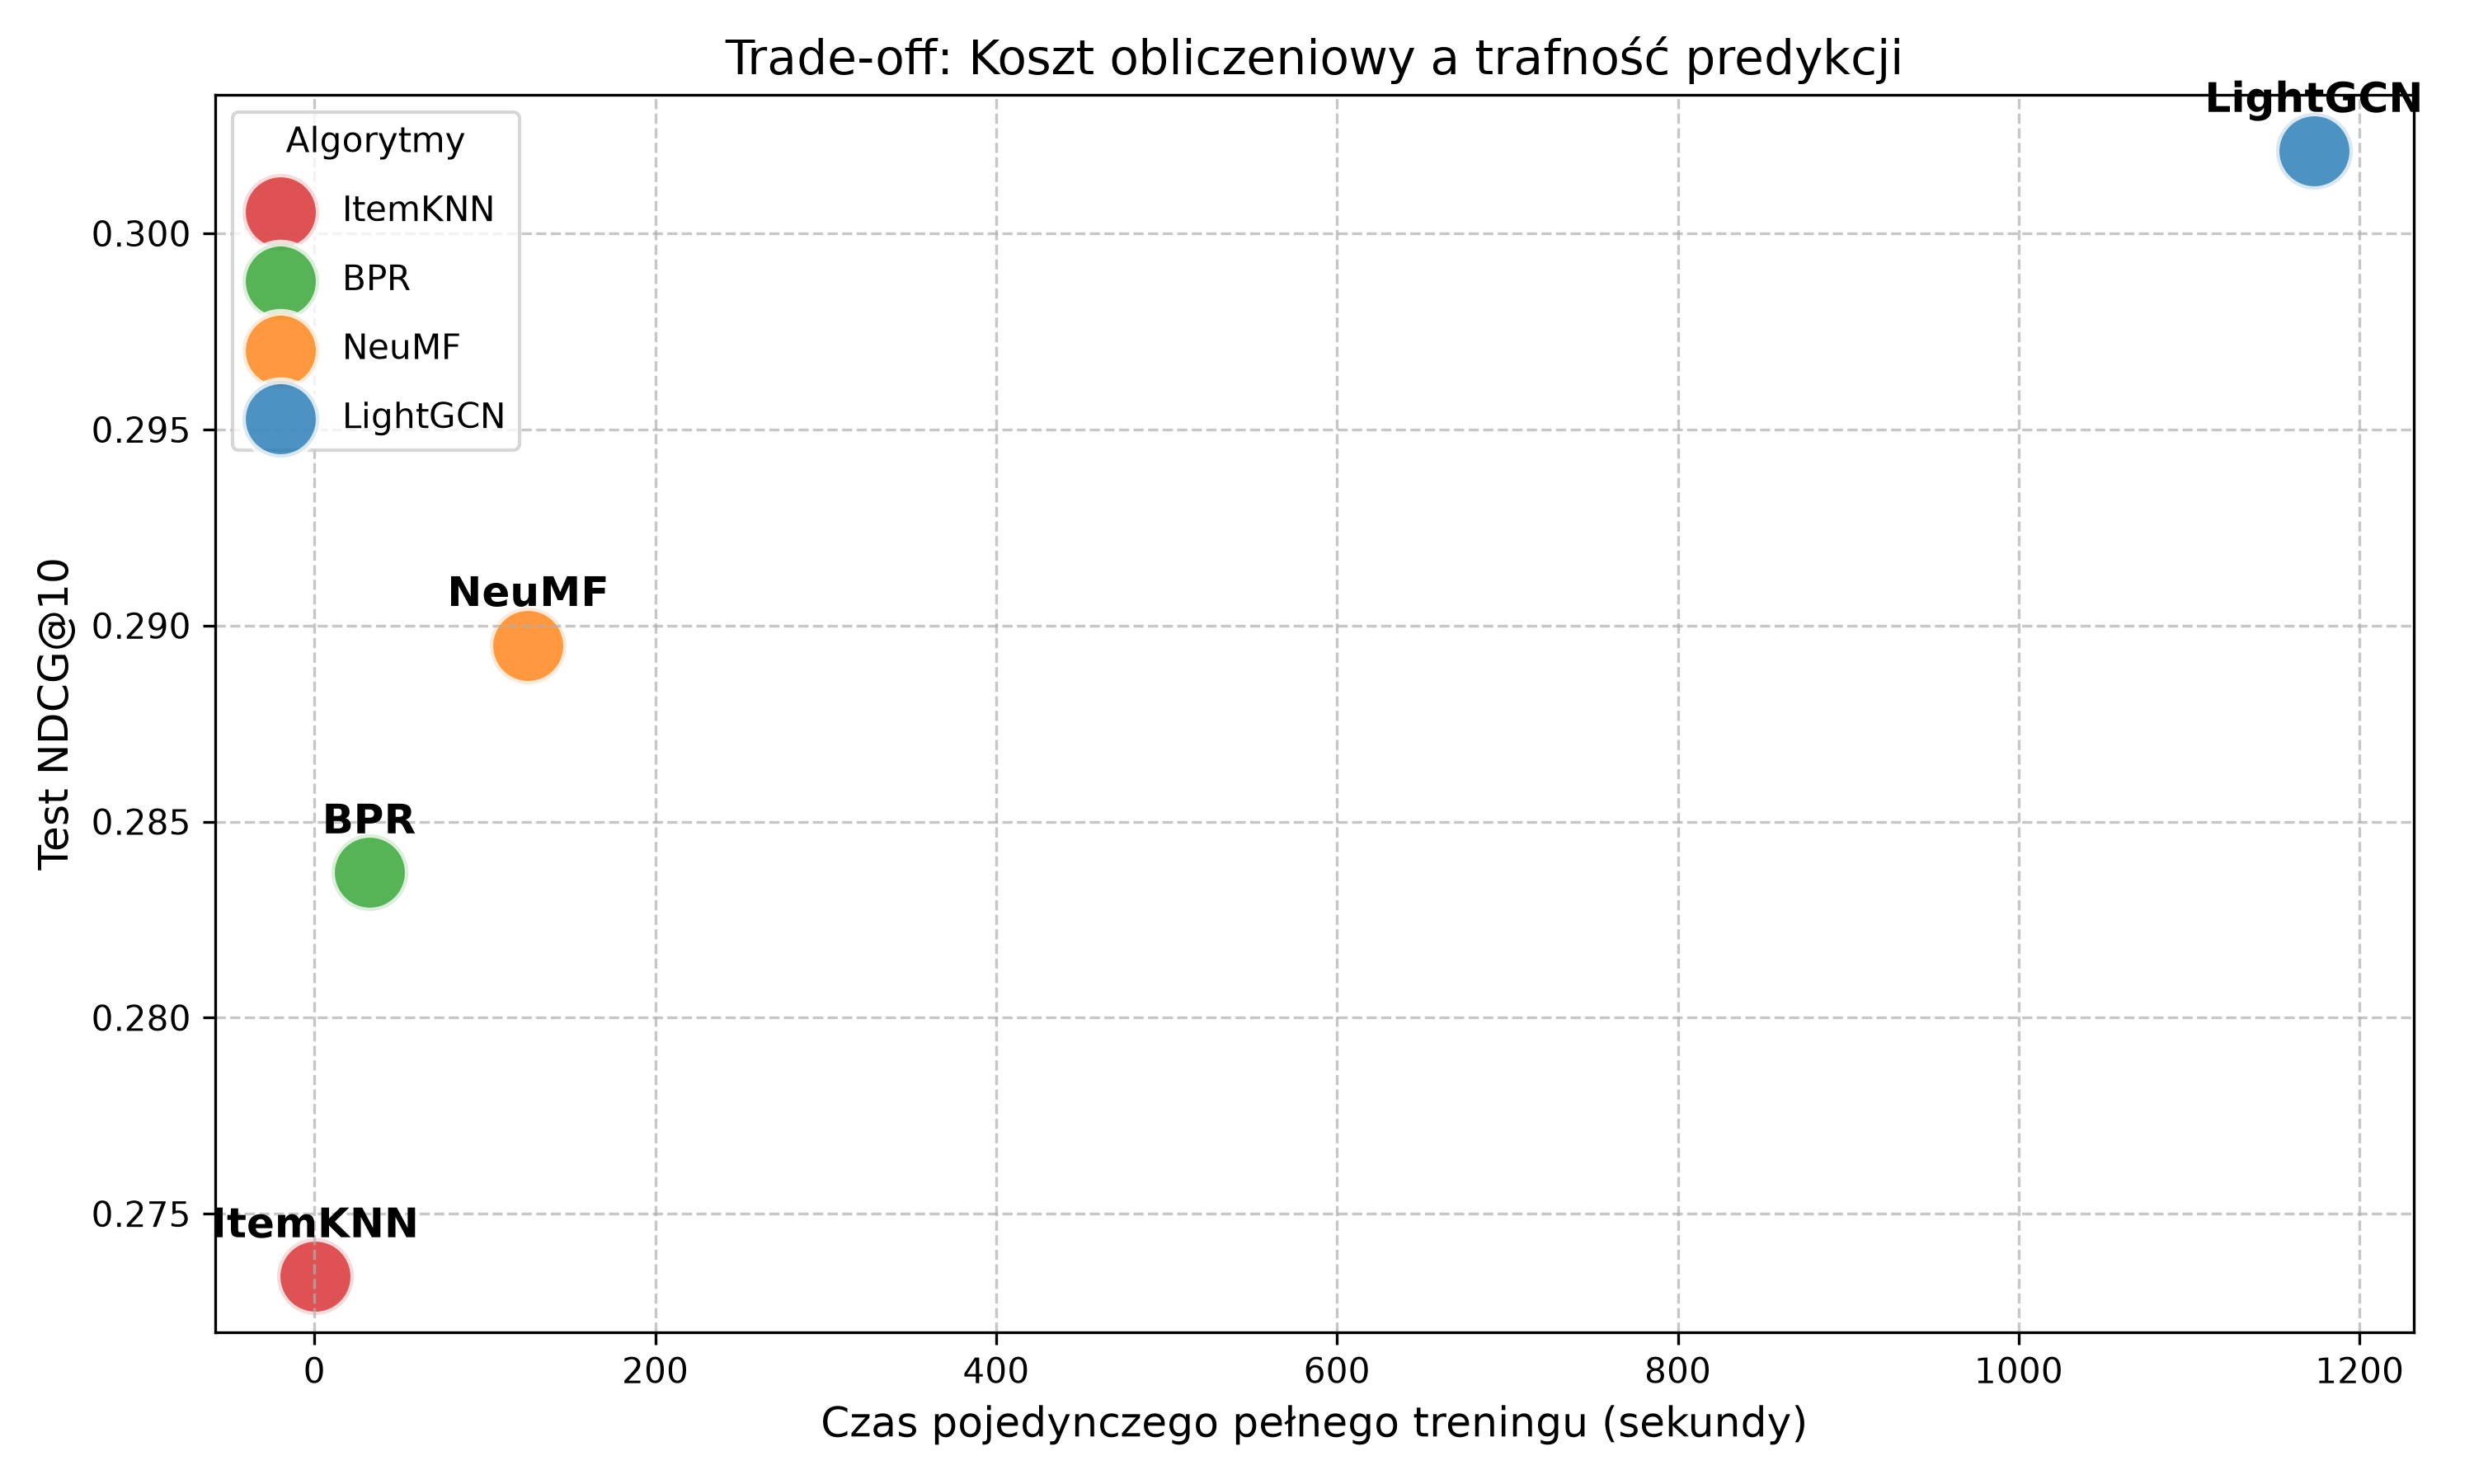
\includegraphics[width=0.8\textwidth]{img/time_vs_ndcg.png}
    \caption[Zestawienie czasu uczenia względem ostatecznej skuteczności dla badanych modeli.]{Zestawienie czasu uczenia względem ostatecznej skuteczności (NDCG@10) dla badanych modeli.}
    \label{fig:time_vs_ndcg}
    \vspace{0.2cm}\noindent{\raggedright \small \textbf{Źródło:} opracowanie własne.\par}
\end{figure}

Wykres punktowy ukazuje bardzo wyraźny kompromis pomiędzy kosztem a jakością. Model bazowy ItemKNN, nie wymagający iteracyjnej optymalizacji stochastycznej, zapewnia bardzo krótki czas odpowiedzi przy relatywnie najniższej skuteczności. Klasyczny wariant BPR jawi się jako algorytm niezwykle efektywny kosztowo. Czas jego uczenia zamyka się w kilkudziesięciu sekundach, dostarczając bardzo zadowalające rezultaty.

Najważniejszym wnioskiem jest jednak ewaluacja grafowych sieci neuronowych. Choć LightGCN przewyższa pozostałe modele pod kątem metryki NDCG, to odbywa się to znacznym kosztem sprzętowym. Czas jego pełnego treningu okazał się niemal 10-krotnie wyższy niż w przypadku głębokiej sieci neuronowej (NeuMF) oraz rzędy wielkości wyższy w porównaniu do klasycznej faktoryzacji macierzy. Wynik ten wskazuje na potencjalne ograniczenia wdrożeniowe algorytmu w czasie rzeczywistym.

\subsection{Dyskusja wyników i wnioski}

Przeprowadzone badania eksperymentalne na zbiorze MovieLens 100K dostarczyły dowodów na to, że ewolucja systemów rekomendacyjnych w kierunku architektur uwzględniających szerszy kontekst powiązań pomiędzy obiektami jest kierunkiem gwarantującym stosunkowo najlepsze wyniki. Metryki rangowe potwierdziły teoretyczną hierarchię modeli, układając się w czytelny ciąg rosnącej skuteczności: od najprostszych metod opartych na pamięci (ItemKNN), poprzez klasyczną faktoryzację macierzy (BPR), głębokie sieci neuronowe (NeuMF), aż po grafowe sieci neuronowe (LightGCN).

Zwycięstwo algorytmu LightGCN we wskaźnikach uwzględniających pozycje w rankingu (NDCG@10 na poziomie 0.3021 oraz MRR@10 wynoszące 0.4835) bezpośrednio udowadnia, że jawne włączenie struktury grafu dwudzielnego do procesu uczenia pozwala na najtrafniejsze ułożenie samej czołówki listy rekomendacji. Jest to zjawisko wysoce pożądane w systemach VOD, gdzie uwaga widza skupia się na pierwszych kilku propozycjach wyświetlanych na ekranie telewizora. Interesującą obserwacją okazał się jednak wynik wskaźnika HR@10, w którym to głęboka architektura NeuMF (0.7720) zdołała nieznacznie wyprzedzić wariant grafowy (0.7678). Sugeruje to, że nieliniowe sieci wielowarstwowe wykazują zdolność do odnajdywania jakiegokolwiek trafnego obiektu i wyprowadzania go do pierwszej dziesiątki, jednak brakuje im precyzji strukturalnej (którą posiada LightGCN), aby wywindować obiekt na wyższe miejsce w rankingu.

Z inżynieryjnego i biznesowego punktu widzenia ostateczne wnioski z badań nie są jednak tak jednoznaczne, jak wskazywałyby na to same miary trafności. Analiza relacji kosztów do jakości (zob. Rysunek \ref{fig:time_vs_ndcg}) pokazała, że zastosowanie najnowocześniejszych rozwiązań opartych na propagacji wiadomości w grafie powoduje znaczny wzrost czasu uczenia. Fakt, iż trening modelu LightGCN wymagał nieporównywalnie więcej nakładów niż optymalizacja wariantu NeuMF, a tym bardziej klasycznego BPR, stanowi zauważalną barierę wdrożeniową. Na wielkoskalowych platformach streamingowych generujących setki milionów logów dziennie proces ten może okazać się problematyczny.

Podsumowując, problematyka wyboru optymalnego algorytmu na rynku komercyjnych usług dostarczania treści wideo nie powinna sprowadzać się wyłącznie do bezwzględnego pościgu za metryką NDCG. Uzyskane wyniki eksperymentalne wskazują, że chociaż grafowe sieci neuronowe bez wątpienia dostarczają obecnie najlepsze wyniki, to w realiach ograniczonego budżetu operacyjnego, drogiej infrastruktury chmurowej oraz wymogu wysokiej responsywności, rozwiązania klasyczne, takie jak zoptymalizowane podejście parowe (BPR) lub architektury hybrydowe (NeuMF), wciąż stanowią niezwykle opłacalną alternatywę.
% !TEX root = ../PRACA_MAIN.tex
\section*{Zakończenie} \addcontentsline{toc}{section}{Zakończenie}

Głównym problemem badawczym podjętym w niniejszej pracy było zjawisko przeciążenia poznawczego na platformach VOD oraz konieczność doboru optymalnych metod zautomatyzowanej personalizacji treści. Celem pracy było kompleksowe porównanie skuteczności różnorodnych algorytmów rekomendacyjnych, wywodzących się z trzech odmiennych paradygmatów: klasycznego filtrowania kolaboracyjnego, architektur uczenia głębokiego oraz nowoczesnych grafowych sieci neuronowych. Główna hipoteza badawcza zakładała, że zaawansowane modele uwzględniające nieliniowość i grafową topologię powiązań (takie jak NeuMF i LightGCN) wykażą znaczącą przewagę predykcyjną nad tradycyjnymi metodami opartymi na faktoryzacji macierzy i sąsiedztwie (ItemKNN, BPR), jednak odbędzie się to kosztem wymiernie wyższego narzutu obliczeniowego.

Przeprowadzone eksperymenty numeryczne na zbiorze danych MovieLens w pełni potwierdziły słuszność przyjętych założeń. Wyniki analiz jednoznacznie wykazały, że ewolucja architektur w kierunku bezpośredniego modelowania struktury grafu dwudzielnego przynosi wymierne korzyści w jakości rekomendacji. Model LightGCN osiągnął najwyższe wyniki w zestawieniu testowym pod kątem kluczowych metryk rangowych (w tym NDCG oraz MRR), udowadniając swoją wysoką zdolność do pozycjonowania najbardziej relewantnych obiektów na samym szczycie listy rekomendacyjnej. Z kolei hybrydowa architektura głęboka NeuMF okazała się najskuteczniejsza w ogólnym odnajdywaniu pożądanych pozycji, osiągając najwyższą wartość wskaźnika trafień. Jednocześnie zidentyfikowano i udokumentowano wyraźny kompromis pomiędzy precyzją układania rankingu a wymaganym czasem uczenia algorytmów. Nowoczesne sieci grafowe wymagały rzędy wielkości dłuższej optymalizacji niż klasyczne metody bazowe.

Biorąc pod uwagę uzyskane wyniki, można stwierdzić, że teza badawcza postawiona we wstępie pracy została udowodniona. Zrealizowano również główny cel badawczy, którym było praktyczne przetestowanie i porównanie wybranych algorytmów pod kątem ich trafności oraz obciążenia sprzętowego w kontekście platform streamingowych.

Wnioski płynące z przeprowadzonych badań posiadają istotne znaczenie praktyczne dla współczesnych przedsiębiorstw działających na rynku. Z biznesowego punktu widzenia wdrożenie najbardziej zaawansowanych algorytmów grafowych bez rzetelnej analizy opłacalności wiązałoby się ze znacznymi kosztami infrastrukturalnymi, które mogą być nieopłacalne w środowiskach wymagających błyskawicznego odświeżania bazy modeli. Przeprowadzona dyskusja wykazała, że w realiach ograniczonych zasobów sprzętowych starsza klasyczna faktoryzacja macierzy (BPR) lub głęboki model NeuMF stanowią wysoce pożądany balans pomiędzy satysfakcją końcowego odbiorcy a kosztami operacyjnymi utrzymania systemu.

Warto jednocześnie podkreślić pewne ograniczenia przeprowadzonych eksperymentów. Z uwagi na wysoką złożoność obliczeniową algorytmów opartych na grafowych sieciach neuronowych oraz ograniczone zasoby sprzętowe, analizę zrealizowano na podzbiorze MovieLens 100K. Wykorzystanie pełnoskalowych, komercyjnych zbiorów danych o znacznie większej rzadkości interakcji mogłoby dodatkowo uwydatnić różnice w precyzji pomiędzy architekturami, a jednocześnie wymusić zastosowanie bardziej wyrafinowanych strategii optymalizacyjnych niż klasyczne przeszukiwanie siatki. Kwestia ta stanowi naturalny kierunek dla przyszłych prac badawczych w tym obszarze.

\printbibliography[notkeyword=internet, heading=bibintoc, title={Bibliografia}]
\printbibliography[keyword=internet, heading=bibintoc, title={Źródła internetowe}]

\newpage
\phantomsection
\addcontentsline{toc}{section}{\listtablename}
\listoftables

\newpage
\phantomsection
\addcontentsline{toc}{section}{\listfigurename}
\listoffigures

\end{document}
